% Created by tikzDevice version 0.12
% !TEX encoding = UTF-8 Unicode
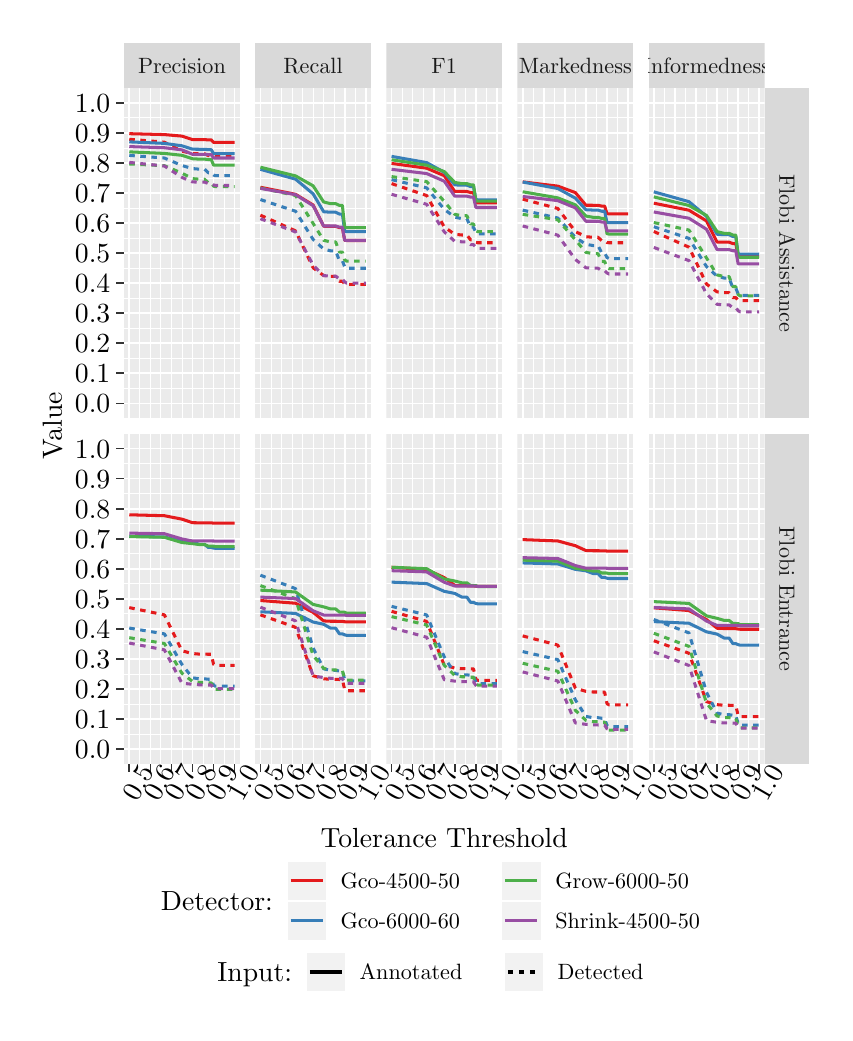
\begin{tikzpicture}[x=1pt,y=1pt]
\definecolor{fillColor}{RGB}{255,255,255}
\path[use as bounding box,fill=fillColor,fill opacity=0.00] (0,0) rectangle (288.00,355.97);
\begin{scope}
\path[clip] (  0.00,  0.00) rectangle (288.00,355.97);
\definecolor{drawColor}{RGB}{255,255,255}
\definecolor{fillColor}{RGB}{255,255,255}

\path[draw=drawColor,line width= 0.6pt,line join=round,line cap=round,fill=fillColor] (  0.00,  0.00) rectangle (288.00,355.97);
\end{scope}
\begin{scope}
\path[clip] ( 34.81,214.79) rectangle ( 76.69,334.21);
\definecolor{fillColor}{gray}{0.92}

\path[fill=fillColor] ( 34.81,214.79) rectangle ( 76.69,334.21);
\definecolor{drawColor}{RGB}{255,255,255}

\path[draw=drawColor,line width= 0.3pt,line join=round] ( 34.81,225.65) --
	( 76.69,225.65);

\path[draw=drawColor,line width= 0.3pt,line join=round] ( 34.81,236.51) --
	( 76.69,236.51);

\path[draw=drawColor,line width= 0.3pt,line join=round] ( 34.81,247.36) --
	( 76.69,247.36);

\path[draw=drawColor,line width= 0.3pt,line join=round] ( 34.81,258.22) --
	( 76.69,258.22);

\path[draw=drawColor,line width= 0.3pt,line join=round] ( 34.81,269.08) --
	( 76.69,269.08);

\path[draw=drawColor,line width= 0.3pt,line join=round] ( 34.81,279.93) --
	( 76.69,279.93);

\path[draw=drawColor,line width= 0.3pt,line join=round] ( 34.81,290.79) --
	( 76.69,290.79);

\path[draw=drawColor,line width= 0.3pt,line join=round] ( 34.81,301.64) --
	( 76.69,301.64);

\path[draw=drawColor,line width= 0.3pt,line join=round] ( 34.81,312.50) --
	( 76.69,312.50);

\path[draw=drawColor,line width= 0.3pt,line join=round] ( 34.81,323.36) --
	( 76.69,323.36);

\path[draw=drawColor,line width= 0.3pt,line join=round] ( 40.52,214.79) --
	( 40.52,334.21);

\path[draw=drawColor,line width= 0.3pt,line join=round] ( 44.33,214.79) --
	( 44.33,334.21);

\path[draw=drawColor,line width= 0.3pt,line join=round] ( 48.13,214.79) --
	( 48.13,334.21);

\path[draw=drawColor,line width= 0.3pt,line join=round] ( 51.94,214.79) --
	( 51.94,334.21);

\path[draw=drawColor,line width= 0.3pt,line join=round] ( 55.75,214.79) --
	( 55.75,334.21);

\path[draw=drawColor,line width= 0.3pt,line join=round] ( 63.37,214.79) --
	( 63.37,334.21);

\path[draw=drawColor,line width= 0.3pt,line join=round] ( 70.98,214.79) --
	( 70.98,334.21);

\path[draw=drawColor,line width= 0.6pt,line join=round] ( 34.81,220.22) --
	( 76.69,220.22);

\path[draw=drawColor,line width= 0.6pt,line join=round] ( 34.81,231.08) --
	( 76.69,231.08);

\path[draw=drawColor,line width= 0.6pt,line join=round] ( 34.81,241.93) --
	( 76.69,241.93);

\path[draw=drawColor,line width= 0.6pt,line join=round] ( 34.81,252.79) --
	( 76.69,252.79);

\path[draw=drawColor,line width= 0.6pt,line join=round] ( 34.81,263.65) --
	( 76.69,263.65);

\path[draw=drawColor,line width= 0.6pt,line join=round] ( 34.81,274.50) --
	( 76.69,274.50);

\path[draw=drawColor,line width= 0.6pt,line join=round] ( 34.81,285.36) --
	( 76.69,285.36);

\path[draw=drawColor,line width= 0.6pt,line join=round] ( 34.81,296.22) --
	( 76.69,296.22);

\path[draw=drawColor,line width= 0.6pt,line join=round] ( 34.81,307.07) --
	( 76.69,307.07);

\path[draw=drawColor,line width= 0.6pt,line join=round] ( 34.81,317.93) --
	( 76.69,317.93);

\path[draw=drawColor,line width= 0.6pt,line join=round] ( 34.81,328.79) --
	( 76.69,328.79);

\path[draw=drawColor,line width= 0.6pt,line join=round] ( 36.71,214.79) --
	( 36.71,334.21);

\path[draw=drawColor,line width= 0.6pt,line join=round] ( 44.33,214.79) --
	( 44.33,334.21);

\path[draw=drawColor,line width= 0.6pt,line join=round] ( 51.94,214.79) --
	( 51.94,334.21);

\path[draw=drawColor,line width= 0.6pt,line join=round] ( 59.56,214.79) --
	( 59.56,334.21);

\path[draw=drawColor,line width= 0.6pt,line join=round] ( 67.17,214.79) --
	( 67.17,334.21);

\path[draw=drawColor,line width= 0.6pt,line join=round] ( 74.79,214.79) --
	( 74.79,334.21);
\definecolor{drawColor}{RGB}{228,26,28}

\path[draw=drawColor,line width= 1.1pt,line join=round] ( 36.71,317.66) --
	( 49.40,317.33) --
	( 55.75,316.78) --
	( 59.56,315.52) --
	( 62.10,315.51) --
	( 63.91,315.51) --
	( 65.27,315.42) --
	( 66.33,315.42) --
	( 67.17,314.52) --
	( 67.87,314.50) --
	( 68.44,314.50) --
	( 74.78,314.50);

\path[draw=drawColor,line width= 1.1pt,dash pattern=on 2pt off 2pt ,line join=round] ( 36.71,315.64) --
	( 49.40,314.60) --
	( 55.75,311.35) --
	( 59.56,310.47) --
	( 62.10,310.38) --
	( 63.91,310.38) --
	( 65.27,309.76) --
	( 66.33,309.76) --
	( 67.17,309.42) --
	( 67.87,309.36) --
	( 68.44,309.36) --
	( 74.78,309.36);
\definecolor{drawColor}{RGB}{55,126,184}

\path[draw=drawColor,line width= 1.1pt,line join=round] ( 36.71,314.70) --
	( 49.40,314.16) --
	( 55.75,313.28) --
	( 59.56,312.06) --
	( 62.10,312.02) --
	( 63.91,312.02) --
	( 65.27,311.89) --
	( 66.33,311.89) --
	( 67.17,310.47) --
	( 67.87,310.45) --
	( 68.44,310.45) --
	( 74.78,310.45);

\path[draw=drawColor,line width= 1.1pt,dash pattern=on 2pt off 2pt ,line join=round] ( 36.71,309.81) --
	( 49.40,308.86) --
	( 55.75,306.15) --
	( 59.56,305.05) --
	( 62.10,304.83) --
	( 63.91,304.83) --
	( 65.27,303.54) --
	( 66.33,303.54) --
	( 67.17,302.70) --
	( 67.87,302.49) --
	( 68.44,302.49) --
	( 74.78,302.49);
\definecolor{drawColor}{RGB}{77,175,74}

\path[draw=drawColor,line width= 1.1pt,line join=round] ( 36.71,311.09) --
	( 49.40,310.53) --
	( 55.75,309.84) --
	( 59.56,308.60) --
	( 62.10,308.46) --
	( 63.91,308.46) --
	( 65.27,308.32) --
	( 66.33,308.32) --
	( 67.17,306.30) --
	( 67.87,306.27) --
	( 68.44,306.27) --
	( 74.78,306.27);

\path[draw=drawColor,line width= 1.1pt,dash pattern=on 2pt off 2pt ,line join=round] ( 36.71,306.72) --
	( 49.40,306.09) --
	( 55.75,303.39) --
	( 59.56,301.42) --
	( 62.10,301.21) --
	( 63.91,301.21) --
	( 65.27,299.86) --
	( 66.33,299.86) --
	( 67.17,298.71) --
	( 67.87,298.52) --
	( 68.44,298.52) --
	( 74.78,298.52);
\definecolor{drawColor}{RGB}{152,78,163}

\path[draw=drawColor,line width= 1.1pt,line join=round] ( 36.71,312.99) --
	( 49.40,312.58) --
	( 55.75,311.82) --
	( 59.56,310.21) --
	( 62.10,310.21) --
	( 63.91,310.21) --
	( 65.27,310.11) --
	( 66.33,310.11) --
	( 67.17,308.87) --
	( 67.87,308.87) --
	( 68.44,308.87) --
	( 74.78,308.87);

\path[draw=drawColor,line width= 1.1pt,dash pattern=on 2pt off 2pt ,line join=round] ( 36.71,307.29) --
	( 49.40,305.98) --
	( 55.75,301.86) --
	( 59.56,300.23) --
	( 62.10,300.15) --
	( 63.91,300.15) --
	( 65.27,299.64) --
	( 66.33,299.64) --
	( 67.17,299.15) --
	( 67.87,298.94) --
	( 68.44,298.94) --
	( 74.78,298.94);
\end{scope}
\begin{scope}
\path[clip] ( 34.81, 89.87) rectangle ( 76.69,209.29);
\definecolor{fillColor}{gray}{0.92}

\path[fill=fillColor] ( 34.81, 89.87) rectangle ( 76.69,209.29);
\definecolor{drawColor}{RGB}{255,255,255}

\path[draw=drawColor,line width= 0.3pt,line join=round] ( 34.81,100.73) --
	( 76.69,100.73);

\path[draw=drawColor,line width= 0.3pt,line join=round] ( 34.81,111.58) --
	( 76.69,111.58);

\path[draw=drawColor,line width= 0.3pt,line join=round] ( 34.81,122.44) --
	( 76.69,122.44);

\path[draw=drawColor,line width= 0.3pt,line join=round] ( 34.81,133.30) --
	( 76.69,133.30);

\path[draw=drawColor,line width= 0.3pt,line join=round] ( 34.81,144.15) --
	( 76.69,144.15);

\path[draw=drawColor,line width= 0.3pt,line join=round] ( 34.81,155.01) --
	( 76.69,155.01);

\path[draw=drawColor,line width= 0.3pt,line join=round] ( 34.81,165.87) --
	( 76.69,165.87);

\path[draw=drawColor,line width= 0.3pt,line join=round] ( 34.81,176.72) --
	( 76.69,176.72);

\path[draw=drawColor,line width= 0.3pt,line join=round] ( 34.81,187.58) --
	( 76.69,187.58);

\path[draw=drawColor,line width= 0.3pt,line join=round] ( 34.81,198.44) --
	( 76.69,198.44);

\path[draw=drawColor,line width= 0.3pt,line join=round] ( 40.52, 89.87) --
	( 40.52,209.29);

\path[draw=drawColor,line width= 0.3pt,line join=round] ( 44.33, 89.87) --
	( 44.33,209.29);

\path[draw=drawColor,line width= 0.3pt,line join=round] ( 48.13, 89.87) --
	( 48.13,209.29);

\path[draw=drawColor,line width= 0.3pt,line join=round] ( 51.94, 89.87) --
	( 51.94,209.29);

\path[draw=drawColor,line width= 0.3pt,line join=round] ( 55.75, 89.87) --
	( 55.75,209.29);

\path[draw=drawColor,line width= 0.3pt,line join=round] ( 63.37, 89.87) --
	( 63.37,209.29);

\path[draw=drawColor,line width= 0.3pt,line join=round] ( 70.98, 89.87) --
	( 70.98,209.29);

\path[draw=drawColor,line width= 0.6pt,line join=round] ( 34.81, 95.30) --
	( 76.69, 95.30);

\path[draw=drawColor,line width= 0.6pt,line join=round] ( 34.81,106.16) --
	( 76.69,106.16);

\path[draw=drawColor,line width= 0.6pt,line join=round] ( 34.81,117.01) --
	( 76.69,117.01);

\path[draw=drawColor,line width= 0.6pt,line join=round] ( 34.81,127.87) --
	( 76.69,127.87);

\path[draw=drawColor,line width= 0.6pt,line join=round] ( 34.81,138.73) --
	( 76.69,138.73);

\path[draw=drawColor,line width= 0.6pt,line join=round] ( 34.81,149.58) --
	( 76.69,149.58);

\path[draw=drawColor,line width= 0.6pt,line join=round] ( 34.81,160.44) --
	( 76.69,160.44);

\path[draw=drawColor,line width= 0.6pt,line join=round] ( 34.81,171.30) --
	( 76.69,171.30);

\path[draw=drawColor,line width= 0.6pt,line join=round] ( 34.81,182.15) --
	( 76.69,182.15);

\path[draw=drawColor,line width= 0.6pt,line join=round] ( 34.81,193.01) --
	( 76.69,193.01);

\path[draw=drawColor,line width= 0.6pt,line join=round] ( 34.81,203.86) --
	( 76.69,203.86);

\path[draw=drawColor,line width= 0.6pt,line join=round] ( 36.71, 89.87) --
	( 36.71,209.29);

\path[draw=drawColor,line width= 0.6pt,line join=round] ( 44.33, 89.87) --
	( 44.33,209.29);

\path[draw=drawColor,line width= 0.6pt,line join=round] ( 51.94, 89.87) --
	( 51.94,209.29);

\path[draw=drawColor,line width= 0.6pt,line join=round] ( 59.56, 89.87) --
	( 59.56,209.29);

\path[draw=drawColor,line width= 0.6pt,line join=round] ( 67.17, 89.87) --
	( 67.17,209.29);

\path[draw=drawColor,line width= 0.6pt,line join=round] ( 74.79, 89.87) --
	( 74.79,209.29);
\definecolor{drawColor}{RGB}{228,26,28}

\path[draw=drawColor,line width= 1.1pt,line join=round] ( 36.71,179.95) --
	( 49.40,179.61) --
	( 55.75,178.37) --
	( 59.56,177.09) --
	( 62.10,177.04) --
	( 63.91,177.04) --
	( 65.27,177.01) --
	( 66.33,177.01) --
	( 67.17,176.95) --
	( 67.87,176.92) --
	( 68.44,176.92) --
	( 74.78,176.92);

\path[draw=drawColor,line width= 1.1pt,dash pattern=on 2pt off 2pt ,line join=round] ( 36.71,146.40) --
	( 49.40,143.78) --
	( 55.75,130.79) --
	( 59.56,129.81) --
	( 62.10,129.60) --
	( 63.91,129.60) --
	( 65.27,129.55) --
	( 66.33,129.55) --
	( 67.17,125.91) --
	( 67.87,125.57) --
	( 68.44,125.57) --
	( 74.78,125.57);
\definecolor{drawColor}{RGB}{55,126,184}

\path[draw=drawColor,line width= 1.1pt,line join=round] ( 36.71,172.20) --
	( 49.40,171.93) --
	( 55.75,170.43) --
	( 59.56,170.02) --
	( 62.10,169.26) --
	( 63.91,169.26) --
	( 65.27,168.14) --
	( 66.33,168.14) --
	( 67.17,167.91) --
	( 67.87,167.83) --
	( 68.44,167.83) --
	( 74.78,167.83);

\path[draw=drawColor,line width= 1.1pt,dash pattern=on 2pt off 2pt ,line join=round] ( 36.71,139.01) --
	( 49.40,136.92) --
	( 55.75,125.86) --
	( 59.56,121.05) --
	( 62.10,120.68) --
	( 63.91,120.68) --
	( 65.27,120.52) --
	( 66.33,120.52) --
	( 67.17,118.35) --
	( 67.87,118.01) --
	( 68.44,118.01) --
	( 74.78,118.01);
\definecolor{drawColor}{RGB}{77,175,74}

\path[draw=drawColor,line width= 1.1pt,line join=round] ( 36.71,172.07) --
	( 49.40,171.82) --
	( 55.75,169.92) --
	( 59.56,169.52) --
	( 62.10,169.18) --
	( 63.91,169.18) --
	( 65.27,168.64) --
	( 66.33,168.64) --
	( 67.17,168.62) --
	( 67.87,168.44) --
	( 68.44,168.44) --
	( 74.78,168.44);

\path[draw=drawColor,line width= 1.1pt,dash pattern=on 2pt off 2pt ,line join=round] ( 36.71,135.53) --
	( 49.40,133.44) --
	( 55.75,122.68) --
	( 59.56,119.74) --
	( 62.10,119.37) --
	( 63.91,119.37) --
	( 65.27,119.22) --
	( 66.33,119.22) --
	( 67.17,117.21) --
	( 67.87,116.88) --
	( 68.44,116.88) --
	( 74.78,116.88);
\definecolor{drawColor}{RGB}{152,78,163}

\path[draw=drawColor,line width= 1.1pt,line join=round] ( 36.71,173.32) --
	( 49.40,173.11) --
	( 55.75,171.21) --
	( 59.56,170.49) --
	( 62.10,170.49) --
	( 63.91,170.49) --
	( 65.27,170.49) --
	( 66.33,170.49) --
	( 67.17,170.48) --
	( 67.87,170.43) --
	( 68.44,170.43) --
	( 74.78,170.43);

\path[draw=drawColor,line width= 1.1pt,dash pattern=on 2pt off 2pt ,line join=round] ( 36.71,133.60) --
	( 49.40,131.14) --
	( 55.75,119.10) --
	( 59.56,118.69) --
	( 62.10,118.51) --
	( 63.91,118.51) --
	( 65.27,118.45) --
	( 66.33,118.45) --
	( 67.17,117.37) --
	( 67.87,117.17) --
	( 68.44,117.17) --
	( 74.78,117.17);
\end{scope}
\begin{scope}
\path[clip] ( 82.19,214.79) rectangle (124.08,334.21);
\definecolor{fillColor}{gray}{0.92}

\path[fill=fillColor] ( 82.19,214.79) rectangle (124.08,334.21);
\definecolor{drawColor}{RGB}{255,255,255}

\path[draw=drawColor,line width= 0.3pt,line join=round] ( 82.19,225.65) --
	(124.08,225.65);

\path[draw=drawColor,line width= 0.3pt,line join=round] ( 82.19,236.51) --
	(124.08,236.51);

\path[draw=drawColor,line width= 0.3pt,line join=round] ( 82.19,247.36) --
	(124.08,247.36);

\path[draw=drawColor,line width= 0.3pt,line join=round] ( 82.19,258.22) --
	(124.08,258.22);

\path[draw=drawColor,line width= 0.3pt,line join=round] ( 82.19,269.08) --
	(124.08,269.08);

\path[draw=drawColor,line width= 0.3pt,line join=round] ( 82.19,279.93) --
	(124.08,279.93);

\path[draw=drawColor,line width= 0.3pt,line join=round] ( 82.19,290.79) --
	(124.08,290.79);

\path[draw=drawColor,line width= 0.3pt,line join=round] ( 82.19,301.64) --
	(124.08,301.64);

\path[draw=drawColor,line width= 0.3pt,line join=round] ( 82.19,312.50) --
	(124.08,312.50);

\path[draw=drawColor,line width= 0.3pt,line join=round] ( 82.19,323.36) --
	(124.08,323.36);

\path[draw=drawColor,line width= 0.3pt,line join=round] ( 87.91,214.79) --
	( 87.91,334.21);

\path[draw=drawColor,line width= 0.3pt,line join=round] ( 91.71,214.79) --
	( 91.71,334.21);

\path[draw=drawColor,line width= 0.3pt,line join=round] ( 95.52,214.79) --
	( 95.52,334.21);

\path[draw=drawColor,line width= 0.3pt,line join=round] ( 99.33,214.79) --
	( 99.33,334.21);

\path[draw=drawColor,line width= 0.3pt,line join=round] (103.14,214.79) --
	(103.14,334.21);

\path[draw=drawColor,line width= 0.3pt,line join=round] (110.75,214.79) --
	(110.75,334.21);

\path[draw=drawColor,line width= 0.3pt,line join=round] (118.37,214.79) --
	(118.37,334.21);

\path[draw=drawColor,line width= 0.6pt,line join=round] ( 82.19,220.22) --
	(124.08,220.22);

\path[draw=drawColor,line width= 0.6pt,line join=round] ( 82.19,231.08) --
	(124.08,231.08);

\path[draw=drawColor,line width= 0.6pt,line join=round] ( 82.19,241.93) --
	(124.08,241.93);

\path[draw=drawColor,line width= 0.6pt,line join=round] ( 82.19,252.79) --
	(124.08,252.79);

\path[draw=drawColor,line width= 0.6pt,line join=round] ( 82.19,263.65) --
	(124.08,263.65);

\path[draw=drawColor,line width= 0.6pt,line join=round] ( 82.19,274.50) --
	(124.08,274.50);

\path[draw=drawColor,line width= 0.6pt,line join=round] ( 82.19,285.36) --
	(124.08,285.36);

\path[draw=drawColor,line width= 0.6pt,line join=round] ( 82.19,296.22) --
	(124.08,296.22);

\path[draw=drawColor,line width= 0.6pt,line join=round] ( 82.19,307.07) --
	(124.08,307.07);

\path[draw=drawColor,line width= 0.6pt,line join=round] ( 82.19,317.93) --
	(124.08,317.93);

\path[draw=drawColor,line width= 0.6pt,line join=round] ( 82.19,328.79) --
	(124.08,328.79);

\path[draw=drawColor,line width= 0.6pt,line join=round] ( 84.10,214.79) --
	( 84.10,334.21);

\path[draw=drawColor,line width= 0.6pt,line join=round] ( 91.71,214.79) --
	( 91.71,334.21);

\path[draw=drawColor,line width= 0.6pt,line join=round] ( 99.33,214.79) --
	( 99.33,334.21);

\path[draw=drawColor,line width= 0.6pt,line join=round] (106.95,214.79) --
	(106.95,334.21);

\path[draw=drawColor,line width= 0.6pt,line join=round] (114.56,214.79) --
	(114.56,334.21);

\path[draw=drawColor,line width= 0.6pt,line join=round] (122.18,214.79) --
	(122.18,334.21);
\definecolor{drawColor}{RGB}{228,26,28}

\path[draw=drawColor,line width= 1.1pt,line join=round] ( 84.10,298.30) --
	( 96.79,295.75) --
	(103.14,291.88) --
	(106.95,284.22) --
	(109.48,284.20) --
	(111.30,284.20) --
	(112.66,283.70) --
	(113.72,283.70) --
	(114.56,279.14) --
	(115.25,279.06) --
	(115.83,279.06) --
	(122.17,279.06);

\path[draw=drawColor,line width= 1.1pt,dash pattern=on 2pt off 2pt ,line join=round] ( 84.10,288.21) --
	( 96.79,282.55) --
	(103.14,269.21) --
	(106.95,266.39) --
	(109.48,266.12) --
	(111.30,266.12) --
	(112.66,264.33) --
	(113.72,264.33) --
	(114.56,263.37) --
	(115.25,263.23) --
	(115.83,263.23) --
	(122.17,263.23);
\definecolor{drawColor}{RGB}{55,126,184}

\path[draw=drawColor,line width= 1.1pt,line join=round] ( 84.10,304.78) --
	( 96.79,301.23) --
	(103.14,295.92) --
	(106.95,289.46) --
	(109.48,289.28) --
	(111.30,289.28) --
	(112.66,288.62) --
	(113.72,288.62) --
	(114.56,282.35) --
	(115.25,282.30) --
	(115.83,282.30) --
	(122.17,282.30);

\path[draw=drawColor,line width= 1.1pt,dash pattern=on 2pt off 2pt ,line join=round] ( 84.10,293.85) --
	( 96.79,289.64) --
	(103.14,279.44) --
	(106.95,275.98) --
	(109.48,275.32) --
	(111.30,275.32) --
	(112.66,271.70) --
	(113.72,271.70) --
	(114.56,269.54) --
	(115.25,269.03) --
	(115.83,269.03) --
	(122.17,269.03);
\definecolor{drawColor}{RGB}{77,175,74}

\path[draw=drawColor,line width= 1.1pt,line join=round] ( 84.10,305.54) --
	( 96.79,302.41) --
	(103.14,298.82) --
	(106.95,292.99) --
	(109.48,292.37) --
	(111.30,292.37) --
	(112.66,291.75) --
	(113.72,291.75) --
	(114.56,283.81) --
	(115.25,283.71) --
	(115.83,283.71) --
	(122.17,283.71);

\path[draw=drawColor,line width= 1.1pt,dash pattern=on 2pt off 2pt ,line join=round] ( 84.10,298.04) --
	( 96.79,295.32) --
	(103.14,285.24) --
	(106.95,279.13) --
	(109.48,278.53) --
	(111.30,278.53) --
	(112.66,274.88) --
	(113.72,274.88) --
	(114.56,272.02) --
	(115.25,271.58) --
	(115.83,271.58) --
	(122.17,271.58);
\definecolor{drawColor}{RGB}{152,78,163}

\path[draw=drawColor,line width= 1.1pt,line join=round] ( 84.10,297.90) --
	( 96.79,295.62) --
	(103.14,291.65) --
	(106.95,284.30) --
	(109.48,284.30) --
	(111.30,284.30) --
	(112.66,283.87) --
	(113.72,283.87) --
	(114.56,279.11) --
	(115.25,279.11) --
	(115.83,279.11) --
	(122.17,279.11);

\path[draw=drawColor,line width= 1.1pt,dash pattern=on 2pt off 2pt ,line join=round] ( 84.10,286.93) --
	( 96.79,282.16) --
	(103.14,270.17) --
	(106.95,266.37) --
	(109.48,266.19) --
	(111.30,266.19) --
	(112.66,265.11) --
	(113.72,265.11) --
	(114.56,264.09) --
	(115.25,263.67) --
	(115.83,263.67) --
	(122.17,263.67);
\end{scope}
\begin{scope}
\path[clip] ( 82.19, 89.87) rectangle (124.08,209.29);
\definecolor{fillColor}{gray}{0.92}

\path[fill=fillColor] ( 82.19, 89.87) rectangle (124.08,209.29);
\definecolor{drawColor}{RGB}{255,255,255}

\path[draw=drawColor,line width= 0.3pt,line join=round] ( 82.19,100.73) --
	(124.08,100.73);

\path[draw=drawColor,line width= 0.3pt,line join=round] ( 82.19,111.58) --
	(124.08,111.58);

\path[draw=drawColor,line width= 0.3pt,line join=round] ( 82.19,122.44) --
	(124.08,122.44);

\path[draw=drawColor,line width= 0.3pt,line join=round] ( 82.19,133.30) --
	(124.08,133.30);

\path[draw=drawColor,line width= 0.3pt,line join=round] ( 82.19,144.15) --
	(124.08,144.15);

\path[draw=drawColor,line width= 0.3pt,line join=round] ( 82.19,155.01) --
	(124.08,155.01);

\path[draw=drawColor,line width= 0.3pt,line join=round] ( 82.19,165.87) --
	(124.08,165.87);

\path[draw=drawColor,line width= 0.3pt,line join=round] ( 82.19,176.72) --
	(124.08,176.72);

\path[draw=drawColor,line width= 0.3pt,line join=round] ( 82.19,187.58) --
	(124.08,187.58);

\path[draw=drawColor,line width= 0.3pt,line join=round] ( 82.19,198.44) --
	(124.08,198.44);

\path[draw=drawColor,line width= 0.3pt,line join=round] ( 87.91, 89.87) --
	( 87.91,209.29);

\path[draw=drawColor,line width= 0.3pt,line join=round] ( 91.71, 89.87) --
	( 91.71,209.29);

\path[draw=drawColor,line width= 0.3pt,line join=round] ( 95.52, 89.87) --
	( 95.52,209.29);

\path[draw=drawColor,line width= 0.3pt,line join=round] ( 99.33, 89.87) --
	( 99.33,209.29);

\path[draw=drawColor,line width= 0.3pt,line join=round] (103.14, 89.87) --
	(103.14,209.29);

\path[draw=drawColor,line width= 0.3pt,line join=round] (110.75, 89.87) --
	(110.75,209.29);

\path[draw=drawColor,line width= 0.3pt,line join=round] (118.37, 89.87) --
	(118.37,209.29);

\path[draw=drawColor,line width= 0.6pt,line join=round] ( 82.19, 95.30) --
	(124.08, 95.30);

\path[draw=drawColor,line width= 0.6pt,line join=round] ( 82.19,106.16) --
	(124.08,106.16);

\path[draw=drawColor,line width= 0.6pt,line join=round] ( 82.19,117.01) --
	(124.08,117.01);

\path[draw=drawColor,line width= 0.6pt,line join=round] ( 82.19,127.87) --
	(124.08,127.87);

\path[draw=drawColor,line width= 0.6pt,line join=round] ( 82.19,138.73) --
	(124.08,138.73);

\path[draw=drawColor,line width= 0.6pt,line join=round] ( 82.19,149.58) --
	(124.08,149.58);

\path[draw=drawColor,line width= 0.6pt,line join=round] ( 82.19,160.44) --
	(124.08,160.44);

\path[draw=drawColor,line width= 0.6pt,line join=round] ( 82.19,171.30) --
	(124.08,171.30);

\path[draw=drawColor,line width= 0.6pt,line join=round] ( 82.19,182.15) --
	(124.08,182.15);

\path[draw=drawColor,line width= 0.6pt,line join=round] ( 82.19,193.01) --
	(124.08,193.01);

\path[draw=drawColor,line width= 0.6pt,line join=round] ( 82.19,203.86) --
	(124.08,203.86);

\path[draw=drawColor,line width= 0.6pt,line join=round] ( 84.10, 89.87) --
	( 84.10,209.29);

\path[draw=drawColor,line width= 0.6pt,line join=round] ( 91.71, 89.87) --
	( 91.71,209.29);

\path[draw=drawColor,line width= 0.6pt,line join=round] ( 99.33, 89.87) --
	( 99.33,209.29);

\path[draw=drawColor,line width= 0.6pt,line join=round] (106.95, 89.87) --
	(106.95,209.29);

\path[draw=drawColor,line width= 0.6pt,line join=round] (114.56, 89.87) --
	(114.56,209.29);

\path[draw=drawColor,line width= 0.6pt,line join=round] (122.18, 89.87) --
	(122.18,209.29);
\definecolor{drawColor}{RGB}{228,26,28}

\path[draw=drawColor,line width= 1.1pt,line join=round] ( 84.10,148.97) --
	( 96.79,147.99) --
	(103.14,144.70) --
	(106.95,141.60) --
	(109.48,141.48) --
	(111.30,141.48) --
	(112.66,141.43) --
	(113.72,141.43) --
	(114.56,141.30) --
	(115.25,141.22) --
	(115.83,141.22) --
	(122.17,141.22);

\path[draw=drawColor,line width= 1.1pt,dash pattern=on 2pt off 2pt ,line join=round] ( 84.10,143.79) --
	( 96.79,139.29) --
	(103.14,121.78) --
	(106.95,120.70) --
	(109.48,120.48) --
	(111.30,120.48) --
	(112.66,120.43) --
	(113.72,120.43) --
	(114.56,116.71) --
	(115.25,116.37) --
	(115.83,116.37) --
	(122.17,116.37);
\definecolor{drawColor}{RGB}{55,126,184}

\path[draw=drawColor,line width= 1.1pt,line join=round] ( 84.10,144.90) --
	( 96.79,144.31) --
	(103.14,141.20) --
	(106.95,140.39) --
	(109.48,138.96) --
	(111.30,138.96) --
	(112.66,136.94) --
	(113.72,136.94) --
	(114.56,136.55) --
	(115.25,136.41) --
	(115.83,136.41) --
	(122.17,136.41);

\path[draw=drawColor,line width= 1.1pt,dash pattern=on 2pt off 2pt ,line join=round] ( 84.10,158.12) --
	( 96.79,153.26) --
	(103.14,131.82) --
	(106.95,124.29) --
	(109.48,123.73) --
	(111.30,123.73) --
	(112.66,123.50) --
	(113.72,123.50) --
	(114.56,120.43) --
	(115.25,119.96) --
	(115.83,119.96) --
	(122.17,119.96);
\definecolor{drawColor}{RGB}{77,175,74}

\path[draw=drawColor,line width= 1.1pt,line join=round] ( 84.10,152.71) --
	( 96.79,152.06) --
	(103.14,147.56) --
	(106.95,146.68) --
	(109.48,145.93) --
	(111.30,145.93) --
	(112.66,144.79) --
	(113.72,144.79) --
	(114.56,144.76) --
	(115.25,144.38) --
	(115.83,144.38) --
	(122.17,144.38);

\path[draw=drawColor,line width= 1.1pt,dash pattern=on 2pt off 2pt ,line join=round] ( 84.10,154.36) --
	( 96.79,149.63) --
	(103.14,129.13) --
	(106.95,124.45) --
	(109.48,123.88) --
	(111.30,123.88) --
	(112.66,123.65) --
	(113.72,123.65) --
	(114.56,120.66) --
	(115.25,120.19) --
	(115.83,120.19) --
	(122.17,120.19);
\definecolor{drawColor}{RGB}{152,78,163}

\path[draw=drawColor,line width= 1.1pt,line join=round] ( 84.10,150.20) --
	( 96.79,149.68) --
	(103.14,145.26) --
	(106.95,143.72) --
	(109.48,143.72) --
	(111.30,143.72) --
	(112.66,143.72) --
	(113.72,143.72) --
	(114.56,143.69) --
	(115.25,143.59) --
	(115.83,143.59) --
	(122.17,143.59);

\path[draw=drawColor,line width= 1.1pt,dash pattern=on 2pt off 2pt ,line join=round] ( 84.10,146.56) --
	( 96.79,141.63) --
	(103.14,121.71) --
	(106.95,121.13) --
	(109.48,120.86) --
	(111.30,120.86) --
	(112.66,120.79) --
	(113.72,120.79) --
	(114.56,119.29) --
	(115.25,119.03) --
	(115.83,119.03) --
	(122.17,119.03);
\end{scope}
\begin{scope}
\path[clip] (129.58,214.79) rectangle (171.47,334.21);
\definecolor{fillColor}{gray}{0.92}

\path[fill=fillColor] (129.58,214.79) rectangle (171.47,334.21);
\definecolor{drawColor}{RGB}{255,255,255}

\path[draw=drawColor,line width= 0.3pt,line join=round] (129.58,225.65) --
	(171.47,225.65);

\path[draw=drawColor,line width= 0.3pt,line join=round] (129.58,236.51) --
	(171.47,236.51);

\path[draw=drawColor,line width= 0.3pt,line join=round] (129.58,247.36) --
	(171.47,247.36);

\path[draw=drawColor,line width= 0.3pt,line join=round] (129.58,258.22) --
	(171.47,258.22);

\path[draw=drawColor,line width= 0.3pt,line join=round] (129.58,269.08) --
	(171.47,269.08);

\path[draw=drawColor,line width= 0.3pt,line join=round] (129.58,279.93) --
	(171.47,279.93);

\path[draw=drawColor,line width= 0.3pt,line join=round] (129.58,290.79) --
	(171.47,290.79);

\path[draw=drawColor,line width= 0.3pt,line join=round] (129.58,301.64) --
	(171.47,301.64);

\path[draw=drawColor,line width= 0.3pt,line join=round] (129.58,312.50) --
	(171.47,312.50);

\path[draw=drawColor,line width= 0.3pt,line join=round] (129.58,323.36) --
	(171.47,323.36);

\path[draw=drawColor,line width= 0.3pt,line join=round] (135.29,214.79) --
	(135.29,334.21);

\path[draw=drawColor,line width= 0.3pt,line join=round] (139.10,214.79) --
	(139.10,334.21);

\path[draw=drawColor,line width= 0.3pt,line join=round] (142.91,214.79) --
	(142.91,334.21);

\path[draw=drawColor,line width= 0.3pt,line join=round] (146.72,214.79) --
	(146.72,334.21);

\path[draw=drawColor,line width= 0.3pt,line join=round] (150.53,214.79) --
	(150.53,334.21);

\path[draw=drawColor,line width= 0.3pt,line join=round] (158.14,214.79) --
	(158.14,334.21);

\path[draw=drawColor,line width= 0.3pt,line join=round] (165.76,214.79) --
	(165.76,334.21);

\path[draw=drawColor,line width= 0.6pt,line join=round] (129.58,220.22) --
	(171.47,220.22);

\path[draw=drawColor,line width= 0.6pt,line join=round] (129.58,231.08) --
	(171.47,231.08);

\path[draw=drawColor,line width= 0.6pt,line join=round] (129.58,241.93) --
	(171.47,241.93);

\path[draw=drawColor,line width= 0.6pt,line join=round] (129.58,252.79) --
	(171.47,252.79);

\path[draw=drawColor,line width= 0.6pt,line join=round] (129.58,263.65) --
	(171.47,263.65);

\path[draw=drawColor,line width= 0.6pt,line join=round] (129.58,274.50) --
	(171.47,274.50);

\path[draw=drawColor,line width= 0.6pt,line join=round] (129.58,285.36) --
	(171.47,285.36);

\path[draw=drawColor,line width= 0.6pt,line join=round] (129.58,296.22) --
	(171.47,296.22);

\path[draw=drawColor,line width= 0.6pt,line join=round] (129.58,307.07) --
	(171.47,307.07);

\path[draw=drawColor,line width= 0.6pt,line join=round] (129.58,317.93) --
	(171.47,317.93);

\path[draw=drawColor,line width= 0.6pt,line join=round] (129.58,328.79) --
	(171.47,328.79);

\path[draw=drawColor,line width= 0.6pt,line join=round] (131.49,214.79) --
	(131.49,334.21);

\path[draw=drawColor,line width= 0.6pt,line join=round] (139.10,214.79) --
	(139.10,334.21);

\path[draw=drawColor,line width= 0.6pt,line join=round] (146.72,214.79) --
	(146.72,334.21);

\path[draw=drawColor,line width= 0.6pt,line join=round] (154.33,214.79) --
	(154.33,334.21);

\path[draw=drawColor,line width= 0.6pt,line join=round] (161.95,214.79) --
	(161.95,334.21);

\path[draw=drawColor,line width= 0.6pt,line join=round] (169.57,214.79) --
	(169.57,334.21);
\definecolor{drawColor}{RGB}{228,26,28}

\path[draw=drawColor,line width= 1.1pt,line join=round] (131.49,306.91) --
	(144.18,305.19) --
	(150.53,302.48) --
	(154.33,296.80) --
	(156.87,296.77) --
	(158.69,296.77) --
	(160.05,296.39) --
	(161.10,296.39) --
	(161.95,292.75) --
	(162.64,292.68) --
	(163.22,292.68) --
	(169.56,292.68);

\path[draw=drawColor,line width= 1.1pt,dash pattern=on 2pt off 2pt ,line join=round] (131.49,299.62) --
	(144.18,295.30) --
	(150.53,283.94) --
	(154.33,281.30) --
	(156.87,281.05) --
	(158.69,281.05) --
	(160.05,279.32) --
	(161.10,279.32) --
	(161.95,278.39) --
	(162.64,278.24) --
	(163.22,278.24) --
	(169.56,278.24);
\definecolor{drawColor}{RGB}{55,126,184}

\path[draw=drawColor,line width= 1.1pt,line join=round] (131.49,309.46) --
	(144.18,307.21) --
	(150.53,303.71) --
	(154.33,299.17) --
	(156.87,299.04) --
	(158.69,299.04) --
	(160.05,298.56) --
	(161.10,298.56) --
	(161.95,293.82) --
	(162.64,293.77) --
	(163.22,293.77) --
	(169.56,293.77);

\path[draw=drawColor,line width= 1.1pt,dash pattern=on 2pt off 2pt ,line join=round] (131.49,301.05) --
	(144.18,298.08) --
	(150.53,290.34) --
	(154.33,287.51) --
	(156.87,286.96) --
	(158.69,286.96) --
	(160.05,283.86) --
	(161.10,283.86) --
	(161.95,281.94) --
	(162.64,281.49) --
	(163.22,281.49) --
	(169.56,281.49);
\definecolor{drawColor}{RGB}{77,175,74}

\path[draw=drawColor,line width= 1.1pt,line join=round] (131.49,308.23) --
	(144.18,306.28) --
	(150.53,303.97) --
	(154.33,300.04) --
	(156.87,299.61) --
	(158.69,299.61) --
	(160.05,299.18) --
	(161.10,299.18) --
	(161.95,293.37) --
	(162.64,293.28) --
	(163.22,293.28) --
	(169.56,293.28);

\path[draw=drawColor,line width= 1.1pt,dash pattern=on 2pt off 2pt ,line join=round] (131.49,302.15) --
	(144.18,300.34) --
	(150.53,293.20) --
	(154.33,288.50) --
	(156.87,288.03) --
	(158.69,288.03) --
	(160.05,285.05) --
	(161.10,285.05) --
	(161.95,282.63) --
	(162.64,282.25) --
	(163.22,282.25) --
	(169.56,282.25);
\definecolor{drawColor}{RGB}{152,78,163}

\path[draw=drawColor,line width= 1.1pt,line join=round] (131.49,304.78) --
	(144.18,303.25) --
	(150.53,300.49) --
	(154.33,295.08) --
	(156.87,295.08) --
	(158.69,295.08) --
	(160.05,294.75) --
	(161.10,294.75) --
	(161.95,290.99) --
	(162.64,290.99) --
	(163.22,290.99) --
	(169.56,290.99);

\path[draw=drawColor,line width= 1.1pt,dash pattern=on 2pt off 2pt ,line join=round] (131.49,295.76) --
	(144.18,292.15) --
	(150.53,282.20) --
	(154.33,278.76) --
	(156.87,278.59) --
	(158.69,278.59) --
	(160.05,277.58) --
	(161.10,277.58) --
	(161.95,276.61) --
	(162.64,276.21) --
	(163.22,276.21) --
	(169.56,276.21);
\end{scope}
\begin{scope}
\path[clip] (129.58, 89.87) rectangle (171.47,209.29);
\definecolor{fillColor}{gray}{0.92}

\path[fill=fillColor] (129.58, 89.87) rectangle (171.47,209.29);
\definecolor{drawColor}{RGB}{255,255,255}

\path[draw=drawColor,line width= 0.3pt,line join=round] (129.58,100.73) --
	(171.47,100.73);

\path[draw=drawColor,line width= 0.3pt,line join=round] (129.58,111.58) --
	(171.47,111.58);

\path[draw=drawColor,line width= 0.3pt,line join=round] (129.58,122.44) --
	(171.47,122.44);

\path[draw=drawColor,line width= 0.3pt,line join=round] (129.58,133.30) --
	(171.47,133.30);

\path[draw=drawColor,line width= 0.3pt,line join=round] (129.58,144.15) --
	(171.47,144.15);

\path[draw=drawColor,line width= 0.3pt,line join=round] (129.58,155.01) --
	(171.47,155.01);

\path[draw=drawColor,line width= 0.3pt,line join=round] (129.58,165.87) --
	(171.47,165.87);

\path[draw=drawColor,line width= 0.3pt,line join=round] (129.58,176.72) --
	(171.47,176.72);

\path[draw=drawColor,line width= 0.3pt,line join=round] (129.58,187.58) --
	(171.47,187.58);

\path[draw=drawColor,line width= 0.3pt,line join=round] (129.58,198.44) --
	(171.47,198.44);

\path[draw=drawColor,line width= 0.3pt,line join=round] (135.29, 89.87) --
	(135.29,209.29);

\path[draw=drawColor,line width= 0.3pt,line join=round] (139.10, 89.87) --
	(139.10,209.29);

\path[draw=drawColor,line width= 0.3pt,line join=round] (142.91, 89.87) --
	(142.91,209.29);

\path[draw=drawColor,line width= 0.3pt,line join=round] (146.72, 89.87) --
	(146.72,209.29);

\path[draw=drawColor,line width= 0.3pt,line join=round] (150.53, 89.87) --
	(150.53,209.29);

\path[draw=drawColor,line width= 0.3pt,line join=round] (158.14, 89.87) --
	(158.14,209.29);

\path[draw=drawColor,line width= 0.3pt,line join=round] (165.76, 89.87) --
	(165.76,209.29);

\path[draw=drawColor,line width= 0.6pt,line join=round] (129.58, 95.30) --
	(171.47, 95.30);

\path[draw=drawColor,line width= 0.6pt,line join=round] (129.58,106.16) --
	(171.47,106.16);

\path[draw=drawColor,line width= 0.6pt,line join=round] (129.58,117.01) --
	(171.47,117.01);

\path[draw=drawColor,line width= 0.6pt,line join=round] (129.58,127.87) --
	(171.47,127.87);

\path[draw=drawColor,line width= 0.6pt,line join=round] (129.58,138.73) --
	(171.47,138.73);

\path[draw=drawColor,line width= 0.6pt,line join=round] (129.58,149.58) --
	(171.47,149.58);

\path[draw=drawColor,line width= 0.6pt,line join=round] (129.58,160.44) --
	(171.47,160.44);

\path[draw=drawColor,line width= 0.6pt,line join=round] (129.58,171.30) --
	(171.47,171.30);

\path[draw=drawColor,line width= 0.6pt,line join=round] (129.58,182.15) --
	(171.47,182.15);

\path[draw=drawColor,line width= 0.6pt,line join=round] (129.58,193.01) --
	(171.47,193.01);

\path[draw=drawColor,line width= 0.6pt,line join=round] (129.58,203.86) --
	(171.47,203.86);

\path[draw=drawColor,line width= 0.6pt,line join=round] (131.49, 89.87) --
	(131.49,209.29);

\path[draw=drawColor,line width= 0.6pt,line join=round] (139.10, 89.87) --
	(139.10,209.29);

\path[draw=drawColor,line width= 0.6pt,line join=round] (146.72, 89.87) --
	(146.72,209.29);

\path[draw=drawColor,line width= 0.6pt,line join=round] (154.33, 89.87) --
	(154.33,209.29);

\path[draw=drawColor,line width= 0.6pt,line join=round] (161.95, 89.87) --
	(161.95,209.29);

\path[draw=drawColor,line width= 0.6pt,line join=round] (169.57, 89.87) --
	(169.57,209.29);
\definecolor{drawColor}{RGB}{228,26,28}

\path[draw=drawColor,line width= 1.1pt,line join=round] (131.49,160.99) --
	(144.18,160.15) --
	(150.53,157.26) --
	(154.33,154.43) --
	(156.87,154.32) --
	(158.69,154.32) --
	(160.05,154.27) --
	(161.10,154.27) --
	(161.95,154.14) --
	(162.64,154.08) --
	(163.22,154.08) --
	(169.56,154.08);

\path[draw=drawColor,line width= 1.1pt,dash pattern=on 2pt off 2pt ,line join=round] (131.49,145.06) --
	(144.18,141.42) --
	(150.53,125.63) --
	(154.33,124.56) --
	(156.87,124.34) --
	(158.69,124.34) --
	(160.05,124.29) --
	(161.10,124.29) --
	(161.95,120.50) --
	(162.64,120.15) --
	(163.22,120.15) --
	(169.56,120.15);
\definecolor{drawColor}{RGB}{55,126,184}

\path[draw=drawColor,line width= 1.1pt,line join=round] (131.49,155.61) --
	(144.18,155.09) --
	(150.53,152.28) --
	(154.33,151.54) --
	(156.87,150.21) --
	(158.69,150.21) --
	(160.05,148.29) --
	(161.10,148.29) --
	(161.95,147.91) --
	(162.64,147.77) --
	(163.22,147.77) --
	(169.56,147.77);

\path[draw=drawColor,line width= 1.1pt,dash pattern=on 2pt off 2pt ,line join=round] (131.49,146.85) --
	(144.18,143.75) --
	(150.53,128.58) --
	(154.33,122.58) --
	(156.87,122.12) --
	(158.69,122.12) --
	(160.05,121.93) --
	(161.10,121.93) --
	(161.95,119.34) --
	(162.64,118.95) --
	(163.22,118.95) --
	(169.56,118.95);
\definecolor{drawColor}{RGB}{77,175,74}

\path[draw=drawColor,line width= 1.1pt,line join=round] (131.49,160.99) --
	(144.18,160.47) --
	(150.53,156.77) --
	(154.33,156.02) --
	(156.87,155.38) --
	(158.69,155.38) --
	(160.05,154.40) --
	(161.10,154.40) --
	(161.95,154.37) --
	(162.64,154.04) --
	(163.22,154.04) --
	(169.56,154.04);

\path[draw=drawColor,line width= 1.1pt,dash pattern=on 2pt off 2pt ,line join=round] (131.49,143.16) --
	(144.18,140.12) --
	(150.53,125.56) --
	(154.33,121.89) --
	(156.87,121.43) --
	(158.69,121.43) --
	(160.05,121.25) --
	(161.10,121.25) --
	(161.95,118.81) --
	(162.64,118.42) --
	(163.22,118.42) --
	(169.56,118.42);
\definecolor{drawColor}{RGB}{152,78,163}

\path[draw=drawColor,line width= 1.1pt,line join=round] (131.49,159.75) --
	(144.18,159.32) --
	(150.53,155.56) --
	(154.33,154.21) --
	(156.87,154.21) --
	(158.69,154.21) --
	(160.05,154.21) --
	(161.10,154.21) --
	(161.95,154.18) --
	(162.64,154.09) --
	(163.22,154.09) --
	(169.56,154.09);

\path[draw=drawColor,line width= 1.1pt,dash pattern=on 2pt off 2pt ,line join=round] (131.49,139.14) --
	(144.18,135.71) --
	(150.53,120.34) --
	(154.33,119.85) --
	(156.87,119.63) --
	(158.69,119.63) --
	(160.05,119.57) --
	(161.10,119.57) --
	(161.95,118.29) --
	(162.64,118.06) --
	(163.22,118.06) --
	(169.56,118.06);
\end{scope}
\begin{scope}
\path[clip] (176.97,214.79) rectangle (218.86,334.21);
\definecolor{fillColor}{gray}{0.92}

\path[fill=fillColor] (176.97,214.79) rectangle (218.86,334.21);
\definecolor{drawColor}{RGB}{255,255,255}

\path[draw=drawColor,line width= 0.3pt,line join=round] (176.97,225.65) --
	(218.86,225.65);

\path[draw=drawColor,line width= 0.3pt,line join=round] (176.97,236.51) --
	(218.86,236.51);

\path[draw=drawColor,line width= 0.3pt,line join=round] (176.97,247.36) --
	(218.86,247.36);

\path[draw=drawColor,line width= 0.3pt,line join=round] (176.97,258.22) --
	(218.86,258.22);

\path[draw=drawColor,line width= 0.3pt,line join=round] (176.97,269.08) --
	(218.86,269.08);

\path[draw=drawColor,line width= 0.3pt,line join=round] (176.97,279.93) --
	(218.86,279.93);

\path[draw=drawColor,line width= 0.3pt,line join=round] (176.97,290.79) --
	(218.86,290.79);

\path[draw=drawColor,line width= 0.3pt,line join=round] (176.97,301.64) --
	(218.86,301.64);

\path[draw=drawColor,line width= 0.3pt,line join=round] (176.97,312.50) --
	(218.86,312.50);

\path[draw=drawColor,line width= 0.3pt,line join=round] (176.97,323.36) --
	(218.86,323.36);

\path[draw=drawColor,line width= 0.3pt,line join=round] (182.68,214.79) --
	(182.68,334.21);

\path[draw=drawColor,line width= 0.3pt,line join=round] (186.49,214.79) --
	(186.49,334.21);

\path[draw=drawColor,line width= 0.3pt,line join=round] (190.30,214.79) --
	(190.30,334.21);

\path[draw=drawColor,line width= 0.3pt,line join=round] (194.11,214.79) --
	(194.11,334.21);

\path[draw=drawColor,line width= 0.3pt,line join=round] (197.91,214.79) --
	(197.91,334.21);

\path[draw=drawColor,line width= 0.3pt,line join=round] (205.53,214.79) --
	(205.53,334.21);

\path[draw=drawColor,line width= 0.3pt,line join=round] (213.15,214.79) --
	(213.15,334.21);

\path[draw=drawColor,line width= 0.6pt,line join=round] (176.97,220.22) --
	(218.86,220.22);

\path[draw=drawColor,line width= 0.6pt,line join=round] (176.97,231.08) --
	(218.86,231.08);

\path[draw=drawColor,line width= 0.6pt,line join=round] (176.97,241.93) --
	(218.86,241.93);

\path[draw=drawColor,line width= 0.6pt,line join=round] (176.97,252.79) --
	(218.86,252.79);

\path[draw=drawColor,line width= 0.6pt,line join=round] (176.97,263.65) --
	(218.86,263.65);

\path[draw=drawColor,line width= 0.6pt,line join=round] (176.97,274.50) --
	(218.86,274.50);

\path[draw=drawColor,line width= 0.6pt,line join=round] (176.97,285.36) --
	(218.86,285.36);

\path[draw=drawColor,line width= 0.6pt,line join=round] (176.97,296.22) --
	(218.86,296.22);

\path[draw=drawColor,line width= 0.6pt,line join=round] (176.97,307.07) --
	(218.86,307.07);

\path[draw=drawColor,line width= 0.6pt,line join=round] (176.97,317.93) --
	(218.86,317.93);

\path[draw=drawColor,line width= 0.6pt,line join=round] (176.97,328.79) --
	(218.86,328.79);

\path[draw=drawColor,line width= 0.6pt,line join=round] (178.87,214.79) --
	(178.87,334.21);

\path[draw=drawColor,line width= 0.6pt,line join=round] (186.49,214.79) --
	(186.49,334.21);

\path[draw=drawColor,line width= 0.6pt,line join=round] (194.11,214.79) --
	(194.11,334.21);

\path[draw=drawColor,line width= 0.6pt,line join=round] (201.72,214.79) --
	(201.72,334.21);

\path[draw=drawColor,line width= 0.6pt,line join=round] (209.34,214.79) --
	(209.34,334.21);

\path[draw=drawColor,line width= 0.6pt,line join=round] (216.95,214.79) --
	(216.95,334.21);
\definecolor{drawColor}{RGB}{228,26,28}

\path[draw=drawColor,line width= 1.1pt,line join=round] (178.87,300.24) --
	(191.57,298.70) --
	(197.91,296.37) --
	(201.72,291.80) --
	(204.26,291.79) --
	(206.07,291.79) --
	(207.43,291.49) --
	(208.49,291.49) --
	(209.34,288.75) --
	(210.03,288.70) --
	(210.61,288.70) --
	(216.95,288.70);

\path[draw=drawColor,line width= 1.1pt,dash pattern=on 2pt off 2pt ,line join=round] (178.87,294.01) --
	(191.57,290.62) --
	(197.91,282.30) --
	(201.72,280.42) --
	(204.26,280.24) --
	(206.07,280.24) --
	(207.43,279.01) --
	(208.49,279.01) --
	(209.34,278.34) --
	(210.03,278.24) --
	(210.61,278.24) --
	(216.95,278.24);
\definecolor{drawColor}{RGB}{55,126,184}

\path[draw=drawColor,line width= 1.1pt,line join=round] (178.87,300.20) --
	(191.57,297.84) --
	(197.91,294.36) --
	(201.72,290.17) --
	(204.26,290.06) --
	(206.07,290.06) --
	(207.43,289.63) --
	(208.49,289.63) --
	(209.34,285.54) --
	(210.03,285.50) --
	(210.61,285.50) --
	(216.95,285.50);

\path[draw=drawColor,line width= 1.1pt,dash pattern=on 2pt off 2pt ,line join=round] (178.87,290.03) --
	(191.57,287.18) --
	(197.91,280.17) --
	(201.72,277.71) --
	(204.26,277.23) --
	(206.07,277.23) --
	(207.43,274.57) --
	(208.49,274.57) --
	(209.34,272.93) --
	(210.03,272.54) --
	(210.61,272.54) --
	(216.95,272.54);
\definecolor{drawColor}{RGB}{77,175,74}

\path[draw=drawColor,line width= 1.1pt,line join=round] (178.87,296.67) --
	(191.57,294.46) --
	(197.91,291.94) --
	(201.72,287.88) --
	(204.26,287.45) --
	(206.07,287.45) --
	(207.43,287.02) --
	(208.49,287.02) --
	(209.34,281.48) --
	(210.03,281.40) --
	(210.61,281.40) --
	(216.95,281.40);

\path[draw=drawColor,line width= 1.1pt,dash pattern=on 2pt off 2pt ,line join=round] (178.87,288.52) --
	(191.57,286.56) --
	(197.91,279.29) --
	(201.72,274.77) --
	(204.26,274.32) --
	(206.07,274.32) --
	(207.43,271.52) --
	(208.49,271.52) --
	(209.34,269.27) --
	(210.03,268.92) --
	(210.61,268.92) --
	(216.95,268.92);
\definecolor{drawColor}{RGB}{152,78,163}

\path[draw=drawColor,line width= 1.1pt,line join=round] (178.87,294.97) --
	(191.57,293.47) --
	(197.91,290.85) --
	(201.72,286.02) --
	(204.26,286.02) --
	(206.07,286.02) --
	(207.43,285.73) --
	(208.49,285.73) --
	(209.34,282.54) --
	(210.03,282.54) --
	(210.61,282.54) --
	(216.95,282.54);

\path[draw=drawColor,line width= 1.1pt,dash pattern=on 2pt off 2pt ,line join=round] (178.87,284.31) --
	(191.57,280.99) --
	(197.91,272.20) --
	(201.72,269.20) --
	(204.26,269.05) --
	(206.07,269.05) --
	(207.43,268.17) --
	(208.49,268.17) --
	(209.34,267.32) --
	(210.03,266.96) --
	(210.61,266.96) --
	(216.95,266.96);
\end{scope}
\begin{scope}
\path[clip] (176.97, 89.87) rectangle (218.86,209.29);
\definecolor{fillColor}{gray}{0.92}

\path[fill=fillColor] (176.97, 89.87) rectangle (218.86,209.29);
\definecolor{drawColor}{RGB}{255,255,255}

\path[draw=drawColor,line width= 0.3pt,line join=round] (176.97,100.73) --
	(218.86,100.73);

\path[draw=drawColor,line width= 0.3pt,line join=round] (176.97,111.58) --
	(218.86,111.58);

\path[draw=drawColor,line width= 0.3pt,line join=round] (176.97,122.44) --
	(218.86,122.44);

\path[draw=drawColor,line width= 0.3pt,line join=round] (176.97,133.30) --
	(218.86,133.30);

\path[draw=drawColor,line width= 0.3pt,line join=round] (176.97,144.15) --
	(218.86,144.15);

\path[draw=drawColor,line width= 0.3pt,line join=round] (176.97,155.01) --
	(218.86,155.01);

\path[draw=drawColor,line width= 0.3pt,line join=round] (176.97,165.87) --
	(218.86,165.87);

\path[draw=drawColor,line width= 0.3pt,line join=round] (176.97,176.72) --
	(218.86,176.72);

\path[draw=drawColor,line width= 0.3pt,line join=round] (176.97,187.58) --
	(218.86,187.58);

\path[draw=drawColor,line width= 0.3pt,line join=round] (176.97,198.44) --
	(218.86,198.44);

\path[draw=drawColor,line width= 0.3pt,line join=round] (182.68, 89.87) --
	(182.68,209.29);

\path[draw=drawColor,line width= 0.3pt,line join=round] (186.49, 89.87) --
	(186.49,209.29);

\path[draw=drawColor,line width= 0.3pt,line join=round] (190.30, 89.87) --
	(190.30,209.29);

\path[draw=drawColor,line width= 0.3pt,line join=round] (194.11, 89.87) --
	(194.11,209.29);

\path[draw=drawColor,line width= 0.3pt,line join=round] (197.91, 89.87) --
	(197.91,209.29);

\path[draw=drawColor,line width= 0.3pt,line join=round] (205.53, 89.87) --
	(205.53,209.29);

\path[draw=drawColor,line width= 0.3pt,line join=round] (213.15, 89.87) --
	(213.15,209.29);

\path[draw=drawColor,line width= 0.6pt,line join=round] (176.97, 95.30) --
	(218.86, 95.30);

\path[draw=drawColor,line width= 0.6pt,line join=round] (176.97,106.16) --
	(218.86,106.16);

\path[draw=drawColor,line width= 0.6pt,line join=round] (176.97,117.01) --
	(218.86,117.01);

\path[draw=drawColor,line width= 0.6pt,line join=round] (176.97,127.87) --
	(218.86,127.87);

\path[draw=drawColor,line width= 0.6pt,line join=round] (176.97,138.73) --
	(218.86,138.73);

\path[draw=drawColor,line width= 0.6pt,line join=round] (176.97,149.58) --
	(218.86,149.58);

\path[draw=drawColor,line width= 0.6pt,line join=round] (176.97,160.44) --
	(218.86,160.44);

\path[draw=drawColor,line width= 0.6pt,line join=round] (176.97,171.30) --
	(218.86,171.30);

\path[draw=drawColor,line width= 0.6pt,line join=round] (176.97,182.15) --
	(218.86,182.15);

\path[draw=drawColor,line width= 0.6pt,line join=round] (176.97,193.01) --
	(218.86,193.01);

\path[draw=drawColor,line width= 0.6pt,line join=round] (176.97,203.86) --
	(218.86,203.86);

\path[draw=drawColor,line width= 0.6pt,line join=round] (178.87, 89.87) --
	(178.87,209.29);

\path[draw=drawColor,line width= 0.6pt,line join=round] (186.49, 89.87) --
	(186.49,209.29);

\path[draw=drawColor,line width= 0.6pt,line join=round] (194.11, 89.87) --
	(194.11,209.29);

\path[draw=drawColor,line width= 0.6pt,line join=round] (201.72, 89.87) --
	(201.72,209.29);

\path[draw=drawColor,line width= 0.6pt,line join=round] (209.34, 89.87) --
	(209.34,209.29);

\path[draw=drawColor,line width= 0.6pt,line join=round] (216.95, 89.87) --
	(216.95,209.29);
\definecolor{drawColor}{RGB}{228,26,28}

\path[draw=drawColor,line width= 1.1pt,line join=round] (178.87,170.98) --
	(191.57,170.49) --
	(197.91,168.77) --
	(201.72,167.02) --
	(204.26,166.96) --
	(206.07,166.96) --
	(207.43,166.92) --
	(208.49,166.92) --
	(209.34,166.85) --
	(210.03,166.80) --
	(210.61,166.80) --
	(216.95,166.80);

\path[draw=drawColor,line width= 1.1pt,dash pattern=on 2pt off 2pt ,line join=round] (178.87,136.18) --
	(191.57,132.86) --
	(197.91,117.29) --
	(201.72,116.15) --
	(204.26,115.91) --
	(206.07,115.91) --
	(207.43,115.85) --
	(208.49,115.85) --
	(209.34,111.68) --
	(210.03,111.29) --
	(210.61,111.29) --
	(216.95,111.29);
\definecolor{drawColor}{RGB}{55,126,184}

\path[draw=drawColor,line width= 1.1pt,line join=round] (178.87,162.55) --
	(191.57,162.19) --
	(197.91,160.23) --
	(201.72,159.70) --
	(204.26,158.73) --
	(206.07,158.73) --
	(207.43,157.31) --
	(208.49,157.31) --
	(209.34,157.03) --
	(210.03,156.93) --
	(210.61,156.93) --
	(216.95,156.93);

\path[draw=drawColor,line width= 1.1pt,dash pattern=on 2pt off 2pt ,line join=round] (178.87,130.51) --
	(191.57,127.61) --
	(197.91,113.06) --
	(201.72,107.09) --
	(204.26,106.63) --
	(206.07,106.63) --
	(207.43,106.43) --
	(208.49,106.43) --
	(209.34,103.80) --
	(210.03,103.39) --
	(210.61,103.39) --
	(216.95,103.39);
\definecolor{drawColor}{RGB}{77,175,74}

\path[draw=drawColor,line width= 1.1pt,line join=round] (178.87,163.56) --
	(191.57,163.20) --
	(197.91,160.62) --
	(201.72,160.09) --
	(204.26,159.63) --
	(206.07,159.63) --
	(207.43,158.92) --
	(208.49,158.92) --
	(209.34,158.90) --
	(210.03,158.66) --
	(210.61,158.66) --
	(216.95,158.66);

\path[draw=drawColor,line width= 1.1pt,dash pattern=on 2pt off 2pt ,line join=round] (178.87,126.29) --
	(191.57,123.40) --
	(197.91,109.30) --
	(201.72,105.64) --
	(204.26,105.18) --
	(206.07,105.18) --
	(207.43,104.99) --
	(208.49,104.99) --
	(209.34,102.52) --
	(210.03,102.13) --
	(210.61,102.13) --
	(216.95,102.13);
\definecolor{drawColor}{RGB}{152,78,163}

\path[draw=drawColor,line width= 1.1pt,line join=round] (178.87,164.45) --
	(191.57,164.16) --
	(197.91,161.60) --
	(201.72,160.65) --
	(204.26,160.65) --
	(206.07,160.65) --
	(207.43,160.65) --
	(208.49,160.65) --
	(209.34,160.63) --
	(210.03,160.57) --
	(210.61,160.57) --
	(216.95,160.57);

\path[draw=drawColor,line width= 1.1pt,dash pattern=on 2pt off 2pt ,line join=round] (178.87,123.16) --
	(191.57,119.88) --
	(197.91,104.73) --
	(201.72,104.23) --
	(204.26,104.00) --
	(206.07,104.00) --
	(207.43,103.94) --
	(208.49,103.94) --
	(209.34,102.63) --
	(210.03,102.39) --
	(210.61,102.39) --
	(216.95,102.39);
\end{scope}
\begin{scope}
\path[clip] (224.36,214.79) rectangle (266.25,334.21);
\definecolor{fillColor}{gray}{0.92}

\path[fill=fillColor] (224.36,214.79) rectangle (266.25,334.21);
\definecolor{drawColor}{RGB}{255,255,255}

\path[draw=drawColor,line width= 0.3pt,line join=round] (224.36,225.65) --
	(266.25,225.65);

\path[draw=drawColor,line width= 0.3pt,line join=round] (224.36,236.51) --
	(266.25,236.51);

\path[draw=drawColor,line width= 0.3pt,line join=round] (224.36,247.36) --
	(266.25,247.36);

\path[draw=drawColor,line width= 0.3pt,line join=round] (224.36,258.22) --
	(266.25,258.22);

\path[draw=drawColor,line width= 0.3pt,line join=round] (224.36,269.08) --
	(266.25,269.08);

\path[draw=drawColor,line width= 0.3pt,line join=round] (224.36,279.93) --
	(266.25,279.93);

\path[draw=drawColor,line width= 0.3pt,line join=round] (224.36,290.79) --
	(266.25,290.79);

\path[draw=drawColor,line width= 0.3pt,line join=round] (224.36,301.64) --
	(266.25,301.64);

\path[draw=drawColor,line width= 0.3pt,line join=round] (224.36,312.50) --
	(266.25,312.50);

\path[draw=drawColor,line width= 0.3pt,line join=round] (224.36,323.36) --
	(266.25,323.36);

\path[draw=drawColor,line width= 0.3pt,line join=round] (230.07,214.79) --
	(230.07,334.21);

\path[draw=drawColor,line width= 0.3pt,line join=round] (233.88,214.79) --
	(233.88,334.21);

\path[draw=drawColor,line width= 0.3pt,line join=round] (237.69,214.79) --
	(237.69,334.21);

\path[draw=drawColor,line width= 0.3pt,line join=round] (241.49,214.79) --
	(241.49,334.21);

\path[draw=drawColor,line width= 0.3pt,line join=round] (245.30,214.79) --
	(245.30,334.21);

\path[draw=drawColor,line width= 0.3pt,line join=round] (252.92,214.79) --
	(252.92,334.21);

\path[draw=drawColor,line width= 0.3pt,line join=round] (260.53,214.79) --
	(260.53,334.21);

\path[draw=drawColor,line width= 0.6pt,line join=round] (224.36,220.22) --
	(266.25,220.22);

\path[draw=drawColor,line width= 0.6pt,line join=round] (224.36,231.08) --
	(266.25,231.08);

\path[draw=drawColor,line width= 0.6pt,line join=round] (224.36,241.93) --
	(266.25,241.93);

\path[draw=drawColor,line width= 0.6pt,line join=round] (224.36,252.79) --
	(266.25,252.79);

\path[draw=drawColor,line width= 0.6pt,line join=round] (224.36,263.65) --
	(266.25,263.65);

\path[draw=drawColor,line width= 0.6pt,line join=round] (224.36,274.50) --
	(266.25,274.50);

\path[draw=drawColor,line width= 0.6pt,line join=round] (224.36,285.36) --
	(266.25,285.36);

\path[draw=drawColor,line width= 0.6pt,line join=round] (224.36,296.22) --
	(266.25,296.22);

\path[draw=drawColor,line width= 0.6pt,line join=round] (224.36,307.07) --
	(266.25,307.07);

\path[draw=drawColor,line width= 0.6pt,line join=round] (224.36,317.93) --
	(266.25,317.93);

\path[draw=drawColor,line width= 0.6pt,line join=round] (224.36,328.79) --
	(266.25,328.79);

\path[draw=drawColor,line width= 0.6pt,line join=round] (226.26,214.79) --
	(226.26,334.21);

\path[draw=drawColor,line width= 0.6pt,line join=round] (233.88,214.79) --
	(233.88,334.21);

\path[draw=drawColor,line width= 0.6pt,line join=round] (241.49,214.79) --
	(241.49,334.21);

\path[draw=drawColor,line width= 0.6pt,line join=round] (249.11,214.79) --
	(249.11,334.21);

\path[draw=drawColor,line width= 0.6pt,line join=round] (256.73,214.79) --
	(256.73,334.21);

\path[draw=drawColor,line width= 0.6pt,line join=round] (264.34,214.79) --
	(264.34,334.21);
\definecolor{drawColor}{RGB}{228,26,28}

\path[draw=drawColor,line width= 1.1pt,line join=round] (226.26,292.55) --
	(238.96,290.00) --
	(245.30,286.13) --
	(249.11,278.48) --
	(251.65,278.45) --
	(253.46,278.45) --
	(254.82,277.95) --
	(255.88,277.95) --
	(256.73,273.39) --
	(257.42,273.31) --
	(258.00,273.31) --
	(264.33,273.31);

\path[draw=drawColor,line width= 1.1pt,dash pattern=on 2pt off 2pt ,line join=round] (226.26,282.31) --
	(238.96,276.65) --
	(245.30,263.31) --
	(249.11,260.49) --
	(251.65,260.22) --
	(253.46,260.22) --
	(254.82,258.43) --
	(255.88,258.43) --
	(256.73,257.47) --
	(257.42,257.33) --
	(258.00,257.33) --
	(264.33,257.33);
\definecolor{drawColor}{RGB}{55,126,184}

\path[draw=drawColor,line width= 1.1pt,line join=round] (226.26,296.65) --
	(238.96,293.09) --
	(245.30,287.79) --
	(249.11,281.33) --
	(251.65,281.15) --
	(253.46,281.15) --
	(254.82,280.49) --
	(255.88,280.49) --
	(256.73,274.22) --
	(257.42,274.17) --
	(258.00,274.17) --
	(264.33,274.17);

\path[draw=drawColor,line width= 1.1pt,dash pattern=on 2pt off 2pt ,line join=round] (226.26,284.03) --
	(238.96,279.82) --
	(245.30,269.62) --
	(249.11,266.16) --
	(251.65,265.50) --
	(253.46,265.50) --
	(254.82,261.88) --
	(255.88,261.88) --
	(256.73,259.72) --
	(257.42,259.21) --
	(258.00,259.21) --
	(264.33,259.21);
\definecolor{drawColor}{RGB}{77,175,74}

\path[draw=drawColor,line width= 1.1pt,line join=round] (226.26,294.83) --
	(238.96,291.70) --
	(245.30,288.10) --
	(249.11,282.27) --
	(251.65,281.65) --
	(253.46,281.65) --
	(254.82,281.04) --
	(255.88,281.04) --
	(256.73,273.10) --
	(257.42,272.99) --
	(258.00,272.99) --
	(264.33,272.99);

\path[draw=drawColor,line width= 1.1pt,dash pattern=on 2pt off 2pt ,line join=round] (226.26,285.55) --
	(238.96,282.82) --
	(245.30,272.74) --
	(249.11,266.63) --
	(251.65,266.03) --
	(253.46,266.03) --
	(254.82,262.38) --
	(255.88,262.38) --
	(256.73,259.53) --
	(257.42,259.08) --
	(258.00,259.08) --
	(264.33,259.08);
\definecolor{drawColor}{RGB}{152,78,163}

\path[draw=drawColor,line width= 1.1pt,line join=round] (226.26,289.37) --
	(238.96,287.10) --
	(245.30,283.12) --
	(249.11,275.78) --
	(251.65,275.78) --
	(253.46,275.78) --
	(254.82,275.35) --
	(255.88,275.35) --
	(256.73,270.58) --
	(257.42,270.58) --
	(258.00,270.58) --
	(264.33,270.58);

\path[draw=drawColor,line width= 1.1pt,dash pattern=on 2pt off 2pt ,line join=round] (226.26,276.56) --
	(238.96,271.79) --
	(245.30,259.80) --
	(249.11,256.00) --
	(251.65,255.82) --
	(253.46,255.82) --
	(254.82,254.74) --
	(255.88,254.74) --
	(256.73,253.72) --
	(257.42,253.30) --
	(258.00,253.30) --
	(264.33,253.30);
\end{scope}
\begin{scope}
\path[clip] (224.36, 89.87) rectangle (266.25,209.29);
\definecolor{fillColor}{gray}{0.92}

\path[fill=fillColor] (224.36, 89.87) rectangle (266.25,209.29);
\definecolor{drawColor}{RGB}{255,255,255}

\path[draw=drawColor,line width= 0.3pt,line join=round] (224.36,100.73) --
	(266.25,100.73);

\path[draw=drawColor,line width= 0.3pt,line join=round] (224.36,111.58) --
	(266.25,111.58);

\path[draw=drawColor,line width= 0.3pt,line join=round] (224.36,122.44) --
	(266.25,122.44);

\path[draw=drawColor,line width= 0.3pt,line join=round] (224.36,133.30) --
	(266.25,133.30);

\path[draw=drawColor,line width= 0.3pt,line join=round] (224.36,144.15) --
	(266.25,144.15);

\path[draw=drawColor,line width= 0.3pt,line join=round] (224.36,155.01) --
	(266.25,155.01);

\path[draw=drawColor,line width= 0.3pt,line join=round] (224.36,165.87) --
	(266.25,165.87);

\path[draw=drawColor,line width= 0.3pt,line join=round] (224.36,176.72) --
	(266.25,176.72);

\path[draw=drawColor,line width= 0.3pt,line join=round] (224.36,187.58) --
	(266.25,187.58);

\path[draw=drawColor,line width= 0.3pt,line join=round] (224.36,198.44) --
	(266.25,198.44);

\path[draw=drawColor,line width= 0.3pt,line join=round] (230.07, 89.87) --
	(230.07,209.29);

\path[draw=drawColor,line width= 0.3pt,line join=round] (233.88, 89.87) --
	(233.88,209.29);

\path[draw=drawColor,line width= 0.3pt,line join=round] (237.69, 89.87) --
	(237.69,209.29);

\path[draw=drawColor,line width= 0.3pt,line join=round] (241.49, 89.87) --
	(241.49,209.29);

\path[draw=drawColor,line width= 0.3pt,line join=round] (245.30, 89.87) --
	(245.30,209.29);

\path[draw=drawColor,line width= 0.3pt,line join=round] (252.92, 89.87) --
	(252.92,209.29);

\path[draw=drawColor,line width= 0.3pt,line join=round] (260.53, 89.87) --
	(260.53,209.29);

\path[draw=drawColor,line width= 0.6pt,line join=round] (224.36, 95.30) --
	(266.25, 95.30);

\path[draw=drawColor,line width= 0.6pt,line join=round] (224.36,106.16) --
	(266.25,106.16);

\path[draw=drawColor,line width= 0.6pt,line join=round] (224.36,117.01) --
	(266.25,117.01);

\path[draw=drawColor,line width= 0.6pt,line join=round] (224.36,127.87) --
	(266.25,127.87);

\path[draw=drawColor,line width= 0.6pt,line join=round] (224.36,138.73) --
	(266.25,138.73);

\path[draw=drawColor,line width= 0.6pt,line join=round] (224.36,149.58) --
	(266.25,149.58);

\path[draw=drawColor,line width= 0.6pt,line join=round] (224.36,160.44) --
	(266.25,160.44);

\path[draw=drawColor,line width= 0.6pt,line join=round] (224.36,171.30) --
	(266.25,171.30);

\path[draw=drawColor,line width= 0.6pt,line join=round] (224.36,182.15) --
	(266.25,182.15);

\path[draw=drawColor,line width= 0.6pt,line join=round] (224.36,193.01) --
	(266.25,193.01);

\path[draw=drawColor,line width= 0.6pt,line join=round] (224.36,203.86) --
	(266.25,203.86);

\path[draw=drawColor,line width= 0.6pt,line join=round] (226.26, 89.87) --
	(226.26,209.29);

\path[draw=drawColor,line width= 0.6pt,line join=round] (233.88, 89.87) --
	(233.88,209.29);

\path[draw=drawColor,line width= 0.6pt,line join=round] (241.49, 89.87) --
	(241.49,209.29);

\path[draw=drawColor,line width= 0.6pt,line join=round] (249.11, 89.87) --
	(249.11,209.29);

\path[draw=drawColor,line width= 0.6pt,line join=round] (256.73, 89.87) --
	(256.73,209.29);

\path[draw=drawColor,line width= 0.6pt,line join=round] (264.34, 89.87) --
	(264.34,209.29);
\definecolor{drawColor}{RGB}{228,26,28}

\path[draw=drawColor,line width= 1.1pt,line join=round] (226.26,146.33) --
	(238.96,145.35) --
	(245.30,142.07) --
	(249.11,138.96) --
	(251.65,138.85) --
	(253.46,138.85) --
	(254.82,138.79) --
	(255.88,138.79) --
	(256.73,138.66) --
	(257.42,138.59) --
	(258.00,138.59) --
	(264.33,138.59);

\path[draw=drawColor,line width= 1.1pt,dash pattern=on 2pt off 2pt ,line join=round] (226.26,134.43) --
	(238.96,129.92) --
	(245.30,112.42) --
	(249.11,111.34) --
	(251.65,111.12) --
	(253.46,111.12) --
	(254.82,111.07) --
	(255.88,111.07) --
	(256.73,107.35) --
	(257.42,107.01) --
	(258.00,107.01) --
	(264.33,107.01);
\definecolor{drawColor}{RGB}{55,126,184}

\path[draw=drawColor,line width= 1.1pt,line join=round] (226.26,141.35) --
	(238.96,140.76) --
	(245.30,137.65) --
	(249.11,136.84) --
	(251.65,135.41) --
	(253.46,135.41) --
	(254.82,133.39) --
	(255.88,133.39) --
	(256.73,133.00) --
	(257.42,132.86) --
	(258.00,132.86) --
	(264.33,132.86);

\path[draw=drawColor,line width= 1.1pt,dash pattern=on 2pt off 2pt ,line join=round] (226.26,142.11) --
	(238.96,137.26) --
	(245.30,115.82) --
	(249.11,108.28) --
	(251.65,107.73) --
	(253.46,107.73) --
	(254.82,107.50) --
	(255.88,107.50) --
	(256.73,104.42) --
	(257.42,103.95) --
	(258.00,103.95) --
	(264.33,103.95);
\definecolor{drawColor}{RGB}{77,175,74}

\path[draw=drawColor,line width= 1.1pt,line join=round] (226.26,148.57) --
	(238.96,147.92) --
	(245.30,143.42) --
	(249.11,142.54) --
	(251.65,141.79) --
	(253.46,141.79) --
	(254.82,140.66) --
	(255.88,140.66) --
	(256.73,140.63) --
	(257.42,140.25) --
	(258.00,140.25) --
	(264.33,140.25);

\path[draw=drawColor,line width= 1.1pt,dash pattern=on 2pt off 2pt ,line join=round] (226.26,137.13) --
	(238.96,132.41) --
	(245.30,111.90) --
	(249.11,107.23) --
	(251.65,106.66) --
	(253.46,106.66) --
	(254.82,106.42) --
	(255.88,106.42) --
	(256.73,103.44) --
	(257.42,102.97) --
	(258.00,102.97) --
	(264.33,102.97);
\definecolor{drawColor}{RGB}{152,78,163}

\path[draw=drawColor,line width= 1.1pt,line join=round] (226.26,146.46) --
	(238.96,145.94) --
	(245.30,141.53) --
	(249.11,139.98) --
	(251.65,139.98) --
	(253.46,139.98) --
	(254.82,139.98) --
	(255.88,139.98) --
	(256.73,139.96) --
	(257.42,139.85) --
	(258.00,139.85) --
	(264.33,139.85);

\path[draw=drawColor,line width= 1.1pt,dash pattern=on 2pt off 2pt ,line join=round] (226.26,130.41) --
	(238.96,125.49) --
	(245.30,105.56) --
	(249.11,104.98) --
	(251.65,104.72) --
	(253.46,104.72) --
	(254.82,104.65) --
	(255.88,104.65) --
	(256.73,103.14) --
	(257.42,102.88) --
	(258.00,102.88) --
	(264.33,102.88);
\end{scope}
\begin{scope}
\path[clip] ( 34.81,334.21) rectangle ( 76.69,350.47);
\definecolor{fillColor}{gray}{0.85}

\path[fill=fillColor] ( 34.81,334.21) rectangle ( 76.69,350.47);
\definecolor{drawColor}{gray}{0.10}

\node[text=drawColor,anchor=base,inner sep=0pt, outer sep=0pt, scale=  0.80] at ( 55.75,339.59) {Precision};
\end{scope}
\begin{scope}
\path[clip] ( 82.19,334.21) rectangle (124.08,350.47);
\definecolor{fillColor}{gray}{0.85}

\path[fill=fillColor] ( 82.19,334.21) rectangle (124.08,350.47);
\definecolor{drawColor}{gray}{0.10}

\node[text=drawColor,anchor=base,inner sep=0pt, outer sep=0pt, scale=  0.80] at (103.14,339.59) {Recall};
\end{scope}
\begin{scope}
\path[clip] (129.58,334.21) rectangle (171.47,350.47);
\definecolor{fillColor}{gray}{0.85}

\path[fill=fillColor] (129.58,334.21) rectangle (171.47,350.47);
\definecolor{drawColor}{gray}{0.10}

\node[text=drawColor,anchor=base,inner sep=0pt, outer sep=0pt, scale=  0.80] at (150.53,339.59) {F1};
\end{scope}
\begin{scope}
\path[clip] (176.97,334.21) rectangle (218.86,350.47);
\definecolor{fillColor}{gray}{0.85}

\path[fill=fillColor] (176.97,334.21) rectangle (218.86,350.47);
\definecolor{drawColor}{gray}{0.10}

\node[text=drawColor,anchor=base,inner sep=0pt, outer sep=0pt, scale=  0.80] at (197.91,339.59) {Markedness};
\end{scope}
\begin{scope}
\path[clip] (224.36,334.21) rectangle (266.25,350.47);
\definecolor{fillColor}{gray}{0.85}

\path[fill=fillColor] (224.36,334.21) rectangle (266.25,350.47);
\definecolor{drawColor}{gray}{0.10}

\node[text=drawColor,anchor=base,inner sep=0pt, outer sep=0pt, scale=  0.80] at (245.30,339.59) {Informedness};
\end{scope}
\begin{scope}
\path[clip] (266.25,214.79) rectangle (282.50,334.21);
\definecolor{fillColor}{gray}{0.85}

\path[fill=fillColor] (266.25,214.79) rectangle (282.50,334.21);
\definecolor{drawColor}{gray}{0.10}

\node[text=drawColor,rotate=-90.00,anchor=base,inner sep=0pt, outer sep=0pt, scale=  0.80] at (271.62,274.50) {Flobi Assistance};
\end{scope}
\begin{scope}
\path[clip] (266.25, 89.87) rectangle (282.50,209.29);
\definecolor{fillColor}{gray}{0.85}

\path[fill=fillColor] (266.25, 89.87) rectangle (282.50,209.29);
\definecolor{drawColor}{gray}{0.10}

\node[text=drawColor,rotate=-90.00,anchor=base,inner sep=0pt, outer sep=0pt, scale=  0.80] at (271.62,149.58) {Flobi Entrance};
\end{scope}
\begin{scope}
\path[clip] (  0.00,  0.00) rectangle (288.00,355.97);
\definecolor{drawColor}{gray}{0.20}

\path[draw=drawColor,line width= 0.6pt,line join=round] ( 36.71, 87.12) --
	( 36.71, 89.87);

\path[draw=drawColor,line width= 0.6pt,line join=round] ( 44.33, 87.12) --
	( 44.33, 89.87);

\path[draw=drawColor,line width= 0.6pt,line join=round] ( 51.94, 87.12) --
	( 51.94, 89.87);

\path[draw=drawColor,line width= 0.6pt,line join=round] ( 59.56, 87.12) --
	( 59.56, 89.87);

\path[draw=drawColor,line width= 0.6pt,line join=round] ( 67.17, 87.12) --
	( 67.17, 89.87);

\path[draw=drawColor,line width= 0.6pt,line join=round] ( 74.79, 87.12) --
	( 74.79, 89.87);
\end{scope}
\begin{scope}
\path[clip] (  0.00,  0.00) rectangle (288.00,355.97);
\definecolor{drawColor}{RGB}{0,0,0}

\node[text=drawColor,rotate= 60.00,anchor=base,inner sep=0pt, outer sep=0pt, scale=  1.00] at ( 42.67, 81.48) {0.5};

\node[text=drawColor,rotate= 60.00,anchor=base,inner sep=0pt, outer sep=0pt, scale=  1.00] at ( 50.29, 81.48) {0.6};

\node[text=drawColor,rotate= 60.00,anchor=base,inner sep=0pt, outer sep=0pt, scale=  1.00] at ( 57.91, 81.48) {0.7};

\node[text=drawColor,rotate= 60.00,anchor=base,inner sep=0pt, outer sep=0pt, scale=  1.00] at ( 65.52, 81.48) {0.8};

\node[text=drawColor,rotate= 60.00,anchor=base,inner sep=0pt, outer sep=0pt, scale=  1.00] at ( 73.14, 81.48) {0.9};

\node[text=drawColor,rotate= 60.00,anchor=base,inner sep=0pt, outer sep=0pt, scale=  1.00] at ( 80.75, 81.48) {1.0};
\end{scope}
\begin{scope}
\path[clip] (  0.00,  0.00) rectangle (288.00,355.97);
\definecolor{drawColor}{gray}{0.20}

\path[draw=drawColor,line width= 0.6pt,line join=round] ( 84.10, 87.12) --
	( 84.10, 89.87);

\path[draw=drawColor,line width= 0.6pt,line join=round] ( 91.71, 87.12) --
	( 91.71, 89.87);

\path[draw=drawColor,line width= 0.6pt,line join=round] ( 99.33, 87.12) --
	( 99.33, 89.87);

\path[draw=drawColor,line width= 0.6pt,line join=round] (106.95, 87.12) --
	(106.95, 89.87);

\path[draw=drawColor,line width= 0.6pt,line join=round] (114.56, 87.12) --
	(114.56, 89.87);

\path[draw=drawColor,line width= 0.6pt,line join=round] (122.18, 87.12) --
	(122.18, 89.87);
\end{scope}
\begin{scope}
\path[clip] (  0.00,  0.00) rectangle (288.00,355.97);
\definecolor{drawColor}{RGB}{0,0,0}

\node[text=drawColor,rotate= 60.00,anchor=base,inner sep=0pt, outer sep=0pt, scale=  1.00] at ( 90.06, 81.48) {0.5};

\node[text=drawColor,rotate= 60.00,anchor=base,inner sep=0pt, outer sep=0pt, scale=  1.00] at ( 97.68, 81.48) {0.6};

\node[text=drawColor,rotate= 60.00,anchor=base,inner sep=0pt, outer sep=0pt, scale=  1.00] at (105.29, 81.48) {0.7};

\node[text=drawColor,rotate= 60.00,anchor=base,inner sep=0pt, outer sep=0pt, scale=  1.00] at (112.91, 81.48) {0.8};

\node[text=drawColor,rotate= 60.00,anchor=base,inner sep=0pt, outer sep=0pt, scale=  1.00] at (120.53, 81.48) {0.9};

\node[text=drawColor,rotate= 60.00,anchor=base,inner sep=0pt, outer sep=0pt, scale=  1.00] at (128.14, 81.48) {1.0};
\end{scope}
\begin{scope}
\path[clip] (  0.00,  0.00) rectangle (288.00,355.97);
\definecolor{drawColor}{gray}{0.20}

\path[draw=drawColor,line width= 0.6pt,line join=round] (131.49, 87.12) --
	(131.49, 89.87);

\path[draw=drawColor,line width= 0.6pt,line join=round] (139.10, 87.12) --
	(139.10, 89.87);

\path[draw=drawColor,line width= 0.6pt,line join=round] (146.72, 87.12) --
	(146.72, 89.87);

\path[draw=drawColor,line width= 0.6pt,line join=round] (154.33, 87.12) --
	(154.33, 89.87);

\path[draw=drawColor,line width= 0.6pt,line join=round] (161.95, 87.12) --
	(161.95, 89.87);

\path[draw=drawColor,line width= 0.6pt,line join=round] (169.57, 87.12) --
	(169.57, 89.87);
\end{scope}
\begin{scope}
\path[clip] (  0.00,  0.00) rectangle (288.00,355.97);
\definecolor{drawColor}{RGB}{0,0,0}

\node[text=drawColor,rotate= 60.00,anchor=base,inner sep=0pt, outer sep=0pt, scale=  1.00] at (137.45, 81.48) {0.5};

\node[text=drawColor,rotate= 60.00,anchor=base,inner sep=0pt, outer sep=0pt, scale=  1.00] at (145.07, 81.48) {0.6};

\node[text=drawColor,rotate= 60.00,anchor=base,inner sep=0pt, outer sep=0pt, scale=  1.00] at (152.68, 81.48) {0.7};

\node[text=drawColor,rotate= 60.00,anchor=base,inner sep=0pt, outer sep=0pt, scale=  1.00] at (160.30, 81.48) {0.8};

\node[text=drawColor,rotate= 60.00,anchor=base,inner sep=0pt, outer sep=0pt, scale=  1.00] at (167.91, 81.48) {0.9};

\node[text=drawColor,rotate= 60.00,anchor=base,inner sep=0pt, outer sep=0pt, scale=  1.00] at (175.53, 81.48) {1.0};
\end{scope}
\begin{scope}
\path[clip] (  0.00,  0.00) rectangle (288.00,355.97);
\definecolor{drawColor}{gray}{0.20}

\path[draw=drawColor,line width= 0.6pt,line join=round] (178.87, 87.12) --
	(178.87, 89.87);

\path[draw=drawColor,line width= 0.6pt,line join=round] (186.49, 87.12) --
	(186.49, 89.87);

\path[draw=drawColor,line width= 0.6pt,line join=round] (194.11, 87.12) --
	(194.11, 89.87);

\path[draw=drawColor,line width= 0.6pt,line join=round] (201.72, 87.12) --
	(201.72, 89.87);

\path[draw=drawColor,line width= 0.6pt,line join=round] (209.34, 87.12) --
	(209.34, 89.87);

\path[draw=drawColor,line width= 0.6pt,line join=round] (216.95, 87.12) --
	(216.95, 89.87);
\end{scope}
\begin{scope}
\path[clip] (  0.00,  0.00) rectangle (288.00,355.97);
\definecolor{drawColor}{RGB}{0,0,0}

\node[text=drawColor,rotate= 60.00,anchor=base,inner sep=0pt, outer sep=0pt, scale=  1.00] at (184.84, 81.48) {0.5};

\node[text=drawColor,rotate= 60.00,anchor=base,inner sep=0pt, outer sep=0pt, scale=  1.00] at (192.45, 81.48) {0.6};

\node[text=drawColor,rotate= 60.00,anchor=base,inner sep=0pt, outer sep=0pt, scale=  1.00] at (200.07, 81.48) {0.7};

\node[text=drawColor,rotate= 60.00,anchor=base,inner sep=0pt, outer sep=0pt, scale=  1.00] at (207.69, 81.48) {0.8};

\node[text=drawColor,rotate= 60.00,anchor=base,inner sep=0pt, outer sep=0pt, scale=  1.00] at (215.30, 81.48) {0.9};

\node[text=drawColor,rotate= 60.00,anchor=base,inner sep=0pt, outer sep=0pt, scale=  1.00] at (222.92, 81.48) {1.0};
\end{scope}
\begin{scope}
\path[clip] (  0.00,  0.00) rectangle (288.00,355.97);
\definecolor{drawColor}{gray}{0.20}

\path[draw=drawColor,line width= 0.6pt,line join=round] (226.26, 87.12) --
	(226.26, 89.87);

\path[draw=drawColor,line width= 0.6pt,line join=round] (233.88, 87.12) --
	(233.88, 89.87);

\path[draw=drawColor,line width= 0.6pt,line join=round] (241.49, 87.12) --
	(241.49, 89.87);

\path[draw=drawColor,line width= 0.6pt,line join=round] (249.11, 87.12) --
	(249.11, 89.87);

\path[draw=drawColor,line width= 0.6pt,line join=round] (256.73, 87.12) --
	(256.73, 89.87);

\path[draw=drawColor,line width= 0.6pt,line join=round] (264.34, 87.12) --
	(264.34, 89.87);
\end{scope}
\begin{scope}
\path[clip] (  0.00,  0.00) rectangle (288.00,355.97);
\definecolor{drawColor}{RGB}{0,0,0}

\node[text=drawColor,rotate= 60.00,anchor=base,inner sep=0pt, outer sep=0pt, scale=  1.00] at (232.23, 81.48) {0.5};

\node[text=drawColor,rotate= 60.00,anchor=base,inner sep=0pt, outer sep=0pt, scale=  1.00] at (239.84, 81.48) {0.6};

\node[text=drawColor,rotate= 60.00,anchor=base,inner sep=0pt, outer sep=0pt, scale=  1.00] at (247.46, 81.48) {0.7};

\node[text=drawColor,rotate= 60.00,anchor=base,inner sep=0pt, outer sep=0pt, scale=  1.00] at (255.07, 81.48) {0.8};

\node[text=drawColor,rotate= 60.00,anchor=base,inner sep=0pt, outer sep=0pt, scale=  1.00] at (262.69, 81.48) {0.9};

\node[text=drawColor,rotate= 60.00,anchor=base,inner sep=0pt, outer sep=0pt, scale=  1.00] at (270.31, 81.48) {1.0};
\end{scope}
\begin{scope}
\path[clip] (  0.00,  0.00) rectangle (288.00,355.97);
\definecolor{drawColor}{RGB}{0,0,0}

\node[text=drawColor,anchor=base east,inner sep=0pt, outer sep=0pt, scale=  1.00] at ( 29.86,216.78) {0.0};

\node[text=drawColor,anchor=base east,inner sep=0pt, outer sep=0pt, scale=  1.00] at ( 29.86,227.63) {0.1};

\node[text=drawColor,anchor=base east,inner sep=0pt, outer sep=0pt, scale=  1.00] at ( 29.86,238.49) {0.2};

\node[text=drawColor,anchor=base east,inner sep=0pt, outer sep=0pt, scale=  1.00] at ( 29.86,249.35) {0.3};

\node[text=drawColor,anchor=base east,inner sep=0pt, outer sep=0pt, scale=  1.00] at ( 29.86,260.20) {0.4};

\node[text=drawColor,anchor=base east,inner sep=0pt, outer sep=0pt, scale=  1.00] at ( 29.86,271.06) {0.5};

\node[text=drawColor,anchor=base east,inner sep=0pt, outer sep=0pt, scale=  1.00] at ( 29.86,281.92) {0.6};

\node[text=drawColor,anchor=base east,inner sep=0pt, outer sep=0pt, scale=  1.00] at ( 29.86,292.77) {0.7};

\node[text=drawColor,anchor=base east,inner sep=0pt, outer sep=0pt, scale=  1.00] at ( 29.86,303.63) {0.8};

\node[text=drawColor,anchor=base east,inner sep=0pt, outer sep=0pt, scale=  1.00] at ( 29.86,314.49) {0.9};

\node[text=drawColor,anchor=base east,inner sep=0pt, outer sep=0pt, scale=  1.00] at ( 29.86,325.34) {1.0};
\end{scope}
\begin{scope}
\path[clip] (  0.00,  0.00) rectangle (288.00,355.97);
\definecolor{drawColor}{gray}{0.20}

\path[draw=drawColor,line width= 0.6pt,line join=round] ( 32.06,220.22) --
	( 34.81,220.22);

\path[draw=drawColor,line width= 0.6pt,line join=round] ( 32.06,231.08) --
	( 34.81,231.08);

\path[draw=drawColor,line width= 0.6pt,line join=round] ( 32.06,241.93) --
	( 34.81,241.93);

\path[draw=drawColor,line width= 0.6pt,line join=round] ( 32.06,252.79) --
	( 34.81,252.79);

\path[draw=drawColor,line width= 0.6pt,line join=round] ( 32.06,263.65) --
	( 34.81,263.65);

\path[draw=drawColor,line width= 0.6pt,line join=round] ( 32.06,274.50) --
	( 34.81,274.50);

\path[draw=drawColor,line width= 0.6pt,line join=round] ( 32.06,285.36) --
	( 34.81,285.36);

\path[draw=drawColor,line width= 0.6pt,line join=round] ( 32.06,296.22) --
	( 34.81,296.22);

\path[draw=drawColor,line width= 0.6pt,line join=round] ( 32.06,307.07) --
	( 34.81,307.07);

\path[draw=drawColor,line width= 0.6pt,line join=round] ( 32.06,317.93) --
	( 34.81,317.93);

\path[draw=drawColor,line width= 0.6pt,line join=round] ( 32.06,328.79) --
	( 34.81,328.79);
\end{scope}
\begin{scope}
\path[clip] (  0.00,  0.00) rectangle (288.00,355.97);
\definecolor{drawColor}{RGB}{0,0,0}

\node[text=drawColor,anchor=base east,inner sep=0pt, outer sep=0pt, scale=  1.00] at ( 29.86, 91.86) {0.0};

\node[text=drawColor,anchor=base east,inner sep=0pt, outer sep=0pt, scale=  1.00] at ( 29.86,102.71) {0.1};

\node[text=drawColor,anchor=base east,inner sep=0pt, outer sep=0pt, scale=  1.00] at ( 29.86,113.57) {0.2};

\node[text=drawColor,anchor=base east,inner sep=0pt, outer sep=0pt, scale=  1.00] at ( 29.86,124.43) {0.3};

\node[text=drawColor,anchor=base east,inner sep=0pt, outer sep=0pt, scale=  1.00] at ( 29.86,135.28) {0.4};

\node[text=drawColor,anchor=base east,inner sep=0pt, outer sep=0pt, scale=  1.00] at ( 29.86,146.14) {0.5};

\node[text=drawColor,anchor=base east,inner sep=0pt, outer sep=0pt, scale=  1.00] at ( 29.86,157.00) {0.6};

\node[text=drawColor,anchor=base east,inner sep=0pt, outer sep=0pt, scale=  1.00] at ( 29.86,167.85) {0.7};

\node[text=drawColor,anchor=base east,inner sep=0pt, outer sep=0pt, scale=  1.00] at ( 29.86,178.71) {0.8};

\node[text=drawColor,anchor=base east,inner sep=0pt, outer sep=0pt, scale=  1.00] at ( 29.86,189.56) {0.9};

\node[text=drawColor,anchor=base east,inner sep=0pt, outer sep=0pt, scale=  1.00] at ( 29.86,200.42) {1.0};
\end{scope}
\begin{scope}
\path[clip] (  0.00,  0.00) rectangle (288.00,355.97);
\definecolor{drawColor}{gray}{0.20}

\path[draw=drawColor,line width= 0.6pt,line join=round] ( 32.06, 95.30) --
	( 34.81, 95.30);

\path[draw=drawColor,line width= 0.6pt,line join=round] ( 32.06,106.16) --
	( 34.81,106.16);

\path[draw=drawColor,line width= 0.6pt,line join=round] ( 32.06,117.01) --
	( 34.81,117.01);

\path[draw=drawColor,line width= 0.6pt,line join=round] ( 32.06,127.87) --
	( 34.81,127.87);

\path[draw=drawColor,line width= 0.6pt,line join=round] ( 32.06,138.73) --
	( 34.81,138.73);

\path[draw=drawColor,line width= 0.6pt,line join=round] ( 32.06,149.58) --
	( 34.81,149.58);

\path[draw=drawColor,line width= 0.6pt,line join=round] ( 32.06,160.44) --
	( 34.81,160.44);

\path[draw=drawColor,line width= 0.6pt,line join=round] ( 32.06,171.30) --
	( 34.81,171.30);

\path[draw=drawColor,line width= 0.6pt,line join=round] ( 32.06,182.15) --
	( 34.81,182.15);

\path[draw=drawColor,line width= 0.6pt,line join=round] ( 32.06,193.01) --
	( 34.81,193.01);

\path[draw=drawColor,line width= 0.6pt,line join=round] ( 32.06,203.86) --
	( 34.81,203.86);
\end{scope}
\begin{scope}
\path[clip] (  0.00,  0.00) rectangle (288.00,355.97);
\definecolor{drawColor}{RGB}{0,0,0}

\node[text=drawColor,anchor=base,inner sep=0pt, outer sep=0pt, scale=  1.00] at (150.53, 59.81) {Tolerance Threshold};
\end{scope}
\begin{scope}
\path[clip] (  0.00,  0.00) rectangle (288.00,355.97);
\definecolor{drawColor}{RGB}{0,0,0}

\node[text=drawColor,rotate= 90.00,anchor=base,inner sep=0pt, outer sep=0pt, scale=  1.00] at ( 12.39,212.04) {Value};
\end{scope}
\begin{scope}
\path[clip] (  0.00,  0.00) rectangle (288.00,355.97);
\definecolor{fillColor}{RGB}{255,255,255}

\path[fill=fillColor] ( 46.16, 23.95) rectangle (254.89, 56.86);
\end{scope}
\begin{scope}
\path[clip] (  0.00,  0.00) rectangle (288.00,355.97);
\definecolor{drawColor}{RGB}{0,0,0}

\node[text=drawColor,anchor=base west,inner sep=0pt, outer sep=0pt, scale=  1.00] at ( 48.16, 36.96) {Detector:};
\end{scope}
\begin{scope}
\path[clip] (  0.00,  0.00) rectangle (288.00,355.97);
\definecolor{drawColor}{RGB}{255,255,255}
\definecolor{fillColor}{gray}{0.95}

\path[draw=drawColor,line width= 0.6pt,line join=round,line cap=round,fill=fillColor] ( 93.60, 40.41) rectangle (108.05, 54.86);
\end{scope}
\begin{scope}
\path[clip] (  0.00,  0.00) rectangle (288.00,355.97);
\definecolor{drawColor}{RGB}{228,26,28}

\path[draw=drawColor,line width= 1.1pt,line join=round] ( 95.04, 47.64) -- (106.60, 47.64);
\end{scope}
\begin{scope}
\path[clip] (  0.00,  0.00) rectangle (288.00,355.97);
\definecolor{drawColor}{RGB}{255,255,255}
\definecolor{fillColor}{gray}{0.95}

\path[draw=drawColor,line width= 0.6pt,line join=round,line cap=round,fill=fillColor] ( 93.60, 25.95) rectangle (108.05, 40.41);
\end{scope}
\begin{scope}
\path[clip] (  0.00,  0.00) rectangle (288.00,355.97);
\definecolor{drawColor}{RGB}{55,126,184}

\path[draw=drawColor,line width= 1.1pt,line join=round] ( 95.04, 33.18) -- (106.60, 33.18);
\end{scope}
\begin{scope}
\path[clip] (  0.00,  0.00) rectangle (288.00,355.97);
\definecolor{drawColor}{RGB}{255,255,255}
\definecolor{fillColor}{gray}{0.95}

\path[draw=drawColor,line width= 0.6pt,line join=round,line cap=round,fill=fillColor] (171.21, 40.41) rectangle (185.66, 54.86);
\end{scope}
\begin{scope}
\path[clip] (  0.00,  0.00) rectangle (288.00,355.97);
\definecolor{drawColor}{RGB}{77,175,74}

\path[draw=drawColor,line width= 1.1pt,line join=round] (172.65, 47.64) -- (184.21, 47.64);
\end{scope}
\begin{scope}
\path[clip] (  0.00,  0.00) rectangle (288.00,355.97);
\definecolor{drawColor}{RGB}{255,255,255}
\definecolor{fillColor}{gray}{0.95}

\path[draw=drawColor,line width= 0.6pt,line join=round,line cap=round,fill=fillColor] (171.21, 25.95) rectangle (185.66, 40.41);
\end{scope}
\begin{scope}
\path[clip] (  0.00,  0.00) rectangle (288.00,355.97);
\definecolor{drawColor}{RGB}{152,78,163}

\path[draw=drawColor,line width= 1.1pt,line join=round] (172.65, 33.18) -- (184.21, 33.18);
\end{scope}
\begin{scope}
\path[clip] (  0.00,  0.00) rectangle (288.00,355.97);
\definecolor{drawColor}{RGB}{0,0,0}

\node[text=drawColor,anchor=base west,inner sep=0pt, outer sep=0pt, scale=  0.80] at (113.05, 44.88) {Gco-4500-50};
\end{scope}
\begin{scope}
\path[clip] (  0.00,  0.00) rectangle (288.00,355.97);
\definecolor{drawColor}{RGB}{0,0,0}

\node[text=drawColor,anchor=base west,inner sep=0pt, outer sep=0pt, scale=  0.80] at (113.05, 30.43) {Gco-6000-60};
\end{scope}
\begin{scope}
\path[clip] (  0.00,  0.00) rectangle (288.00,355.97);
\definecolor{drawColor}{RGB}{0,0,0}

\node[text=drawColor,anchor=base west,inner sep=0pt, outer sep=0pt, scale=  0.80] at (190.66, 44.88) {Grow-6000-50};
\end{scope}
\begin{scope}
\path[clip] (  0.00,  0.00) rectangle (288.00,355.97);
\definecolor{drawColor}{RGB}{0,0,0}

\node[text=drawColor,anchor=base west,inner sep=0pt, outer sep=0pt, scale=  0.80] at (190.66, 30.43) {Shrink-4500-50};
\end{scope}
\begin{scope}
\path[clip] (  0.00,  0.00) rectangle (288.00,355.97);
\definecolor{fillColor}{RGB}{255,255,255}

\path[fill=fillColor] ( 66.56,  5.50) rectangle (234.50, 23.95);
\end{scope}
\begin{scope}
\path[clip] (  0.00,  0.00) rectangle (288.00,355.97);
\definecolor{drawColor}{RGB}{0,0,0}

\node[text=drawColor,anchor=base west,inner sep=0pt, outer sep=0pt, scale=  1.00] at ( 68.56, 11.28) {Input:};
\end{scope}
\begin{scope}
\path[clip] (  0.00,  0.00) rectangle (288.00,355.97);
\definecolor{drawColor}{RGB}{255,255,255}
\definecolor{fillColor}{gray}{0.95}

\path[draw=drawColor,line width= 0.6pt,line join=round,line cap=round,fill=fillColor] (100.49,  7.50) rectangle (114.95, 21.95);
\end{scope}
\begin{scope}
\path[clip] (  0.00,  0.00) rectangle (288.00,355.97);
\definecolor{drawColor}{RGB}{0,0,0}

\path[draw=drawColor,line width= 1.1pt,line join=round] (101.94, 14.73) -- (113.50, 14.73);
\end{scope}
\begin{scope}
\path[clip] (  0.00,  0.00) rectangle (288.00,355.97);
\definecolor{drawColor}{RGB}{255,255,255}
\definecolor{fillColor}{gray}{0.95}

\path[draw=drawColor,line width= 0.6pt,line join=round,line cap=round,fill=fillColor] (172.05,  7.50) rectangle (186.50, 21.95);
\end{scope}
\begin{scope}
\path[clip] (  0.00,  0.00) rectangle (288.00,355.97);
\definecolor{drawColor}{RGB}{0,0,0}

\path[draw=drawColor,line width= 1.1pt,dash pattern=on 2pt off 2pt ,line join=round] (173.50, 14.73) -- (185.06, 14.73);
\end{scope}
\begin{scope}
\path[clip] (  0.00,  0.00) rectangle (288.00,355.97);
\definecolor{drawColor}{RGB}{0,0,0}

\node[text=drawColor,anchor=base west,inner sep=0pt, outer sep=0pt, scale=  0.80] at (119.95, 11.97) {Annotated};
\end{scope}
\begin{scope}
\path[clip] (  0.00,  0.00) rectangle (288.00,355.97);
\definecolor{drawColor}{RGB}{0,0,0}

\node[text=drawColor,anchor=base west,inner sep=0pt, outer sep=0pt, scale=  0.80] at (191.50, 11.97) {Detected};
\end{scope}
\end{tikzpicture}
